%%%%%%%%%%%%%%%%%%%%%%% file template.tex %%%%%%%%%%%%%%%%%%%%%%%%%
%
% This is a general template file for the LaTeX package SVJour3
% for Springer journals.          Springer Heidelberg 2010/09/16
%
% Copy it to a new file with a new name and use it as the basis
% for your article. Delete % signs as needed.
%
% This template includes a few options for different layouts and
% content for various journals. Please consult a previous issue of
% your journal as needed.
%
%%%%%%%%%%%%%%%%%%%%%%%%%%%%%%%%%%%%%%%%%%%%%%%%%%%%%%%%%%%%%%%%%%%
%
% First comes an example EPS file -- just ignore it and
% proceed on the \documentclass line
% your LaTeX will extract the file if required
%\begin{filecontents*}{example.eps}
%%!PS-Adobe-3.0 EPSF-3.0
%%%BoundingBox: 19 19 221 221
%%%CreationDate: Mon Sep 29 1997
%%%Creator: programmed by hand (JK)
%%%EndComments
%gsave
%newpath
%  20 20 moveto
%  20 220 lineto
%  220 220 lineto
%  220 20 lineto
%closepath
%2 setlinewidth
%gsave
%  .4 setgray fill
%grestore
%stroke
%grestore
%\end{filecontents*}
%
\RequirePackage{fix-cm}
%
\documentclass{svjour3}                     % onecolumn (standard format)
%\documentclass[smallcondensed]{svjour3}     % onecolumn (ditto)
%\documentclass[smallextended]{svjour3}       % onecolumn (second format)
%\documentclass[twocolumn]{svjour3}          % twocolumn
%
\smartqed  % flush right qed marks, e.g. at end of proof
%

\usepackage{graphicx}% Include figure files
\usepackage{epstopdf, epsfig}
\usepackage{dcolumn}% Align table columns on decimal point

%\draft % marks overfull lines with a black rule on the right
\usepackage{amssymb}
\usepackage{amsmath}
%\usepackage{natbib}
\usepackage{subfloat}
\usepackage{subcaption}
\captionsetup{compatibility=false}
\usepackage{bm}% bold math
\graphicspath{{./figures/}}
%%======================New commands============================================
\newcommand{\todo}[1]{\textcolor{magenta}{#1}}
\newcommand{\changes}[1]{\textcolor{magenta}{#1}}     %%defined a new function to trace changes by modfiy font color
\def\vec#1{\mbox{\boldmath $#1$}}
\newcommand{\bu}{\mathbf{u}}
\newcommand{\bw}{\mathbf{w}}
\newcommand{\bn}{\mathbf{n}}
\newcommand{\bnx}{\mathbf{n_x}}
\newcommand{\bny}{\mathbf{n_y}}
\newcommand{\bs}{\boldsymbol{\sigma}}
\newcommand{\disnum}[1]{\texttt{#1}}
\def\Otf{\Omega^\mathrm{f}(t)}
\def\Ots{\Omega^\mathrm{s}(t)}
\def\Of{\Omega^\mathrm{f}}
\def\Os{\Omega^\mathrm{s}}
\def\bz{\mathbf z}
\newcommand{\xx}{\mbox{$\mathbf{x}^{\mathrm{f}}$}}
\def\strain{\vec \epsilon}
\def\stress{{\vec \sigma}}
\def\div{\vec \nabla}
\def\G{\Gamma}
\def\vphi{\vec{\varphi}^\mathrm{s}}
\newcommand{\bchi}{\mathbf{\chi}}

\usepackage{environ}
\NewEnviron{myequation}{%
\begin{equation}
\scalebox{0.7}{$\BODY$}
\end{equation}
}

\usepackage{xcolor}
\usepackage{tikz}

\newcommand{\reddashdot}{\raisebox{2pt}{\tikz{\draw[red,dashdotted,line width=1.2pt](0,0) -- (5mm,0);}}}
\newcommand{\bluedashdot}{\raisebox{2pt}{\tikz{\draw[blue,dashdotted,line width=1.2pt](0,0) -- (5mm,0);}}}
\newcommand{\greendashdot}{\raisebox{2pt}{\tikz{\draw[green,dashdotted,line width=1.2pt](0,0) -- (5mm,0);}}}
\newcommand{\greendash}{\raisebox{2pt}{\tikz{\draw[green,dashed,line width=1.2pt](0,0) -- (5mm,0);}}}
\newcommand{\greensolid}{\raisebox{2pt}{\tikz{\draw[green,solid,line width=1.2pt](0,0) -- (5mm,0);}}}
\newcommand{\reddash}{\raisebox{2pt}{\tikz{\draw[red,dashed,line width=1.2pt](0,0) -- (5mm,0);}}}
\newcommand{\reddot}{\raisebox{2pt}{\tikz{\draw[red,dotted,line width=1.2pt](0,0) -- (5mm,0);}}}
\newcommand{\bluedash}{\raisebox{2pt}{\tikz{\draw[blue,dashed,line width=1.2pt](0,0) -- (5mm,0);}}}
\newcommand{\blackdash}{\raisebox{2pt}{\tikz{\draw[black,dashed,line width=1.2pt](0,0) -- (5mm,0);}}}
\DeclareMathAlphabet{\mathsfbi}{OT1}{\sfdefault}{bx}{sl}
%
% \usepackage{mathptmx}      % use Times fonts if available on your TeX system
%
% insert here the call for the packages your document requires
%\usepackage{latexsym}
% etc.
%
% please place your own definitions here and don't use \def but
% \newcommand{}{}
%
% Insert the name of "your journal" with
% \journalname{myjournal}
%
\begin{document}

\title{Origin of nonlinear wake induced vibration %\thanks{Grants or other notes
%about the article that should go on the front page should be
%placed here. General acknowledgments should be placed at the end of the article.}
}
%\subtitle{Linear stability analysis}

%\titlerunning{Short form of title}        % if too long for running head

\author{W.YAO         \and
        R.K.JAIMAN %etc.
}

%\authorrunning{Short form of author list} % if too long for running head

\institute{W.YAO \at
              National University of Singapore, now at Queen's University Belfast \\
              \email{w.yao@qub.ac.uk}           %  \\
%             \emph{Present address:} of F. Author  %  if needed
           \and
           R.K.JAIMAN \at
              National University of Singapore
}

\date{Received: date / Accepted: date}
% The correct dates will be entered by the editor


\maketitle

\begin{abstract}

We perform linear stability analysis (LSA) for the flow-induced vibration arranged in tandum configuration
or wake induced vibration (WIV). 
The fluid reduced order model (ROM) is constructed by using an eigensysem realization algorithm (ERA) and 
coupled with a transversely vibrating bluff body in a state space format \cite{yao_jfm_1}. The WIV region and onset reduced velocity 
$U_r$ can be predicted acurately by tracing the eigenvalue trajectories of the ROM for a range of $U_r$. 
The LSA reveals that the structure mode is the energy source to maintain WIV for $(Re,L)=(60,2)$, where $L$ is 
the streamwise distance of the two cylinders. The sharp corner of square cylinder 
is found to have the stabilizing effects, therefore, the WIV onset $U_r$ is larger than its circular cylinder counterpart. 
The LSA shows that the circular cylinder WIV persists for $U_r \ge 6.1$, while the WIV of square 
cylinder terminates at $U_r \approx 19$ at $(Re,L)=(60,2)$. 
%%
The work extends our previous understanding of the vortex induced vibration (VIV) lock-in mechanism to
WIV at low Reynolds number and provides an expolation of the origion of WIV and why it persists at certain 
conditons. 
\keywords{Nonlinear \and Wake-induced-vibration \and Model reduction}

\end{abstract}

%%
\section{Introduction}
\label{intro}

% definition  VIV 
vortex induced vibration (VIV) is a complex nonlinear coupling between the structure and the flow dynamic, which 
often results in large motion and reduce the structural fatigue life. 
VIVs have broad interests in the fields of offshore, wind, aerospace and energy harvesting engineering due to 
its richness in fluid physics. In VIV lock-in regime, the vortex shedding frequency deviates from the Strouhal
law and lock on to the structure natural freqency. This freuqncy lock-in phenomenon is typically charaterized by 
high structue amplitude and therefore has been an active topic over the past decade (\cite{sarpkaya2004,Williamson2004,bearman2011}). 

%% VIV mechanism 
The commonly accepted interpretation of VIVs is attributed to the classical resoanance, which depends on 
vortex shedding frequency ($f_{vs}$) matching structure natural frequency ($f_N$). However, numerical simulation has shown that 
the peak amplitude arises in the vicinity of lock-in onset rather than at $f_{vs}/f_N \approx 1$. Recently, Yao and Jaiman \cite{yao_jfm_1} 
developed an efficient VIV reduced order model (ROM) using eigensystem realiation algorith (ERA) and successfully performed
linear stability analysis (LSA) of VIV system. 
The authors show that the lock-in onset of bluff bodies is trigged by unstable structure mode (SM), and 
the low freuqency galloping is characterized by persisting unstable SM. The understanding of lock-in mechanism by ERA-based ROM 
paves a way to develop a feedback control strategy for VIVs suppresion \cite{yao_jfm_2}. 


%%definition WIV 
The wake induced vibration or WIV is considered as the flow induced vibration in tandum 
configuration. The nature of VIV and WIV arises simlarly from wake instability. However, WIV has its particular physics 
feature. Based on spacing to diameter ratio ($L/D$), The tandum cylinder is charaterized by 
three interfernce regimes \cite{Mysa2016,ZDRAVKOVICH1987239,1981323}: proximity interfernce ($1 \le L/D \le 1.2$ to $1.8$), 
wake interference ($1.8 \le L/D \le 3.4$ to $3.8$) and no interfernce ($L/D \ge 3.8$).
In proximity regime, the vortex shedding
from the upstream cylinder is suppressed and the tandum bodyies behave like a single bluff body, whereas the flow becomes intricate 
in wake interference and shear layer reattachment, intermitten vortex shedding, etc gradully appear as $L/D$ increases. 
The no interfernce regime is dominated by the co-shedding, where vortex shedding occurs separately from both the cylinders.

%% WIV mechanism 

The downstream cylinder experiences large response persisting to high reduced velocity 
which is typically defined as wake induced galloping \cite{bokaian1984}. Recent work 
\cite{assi2010} dissocates the WIV from galloping concept. The authors argue the WIV is 
sustained by unsteady vortex shedding that provides energy to the WIV system, 
and has difference mechanism from VIV, which is considered as 
as a \textit{resonance} phenomenon. In another recent work \cite{assi2013}, the authors provided a 
phsical explanation for WIV by wake-stiffness concept. They argued that the wake-stiffness characterizes the 
WIV properties. The authors \cite{assi2010,assi2013} insists that the WIV is a non-resonance 
fluid induced vibration (FIV) with increasing amplituded beyond frequency lock-in regime, and is mainly due to 
unsteady wake. 
%


%%
The paper is organized as follows. Section  \ref{sec:Numeric method} introduceds the FOM, ERA and ERA-based WIV ROM 
formulation in state space format. Section \ref{sec:set-up} describes the problem set-up. The LSA results are discussed 
in section \ref{•}followed by conclusion in \ref{•}. 

\section{Numerical methodology}\label{sec:Numeric method}
\subsection{Full-order model formulation}

Consider the fluid domain $\Otf$ with the spatial and temporal coordinates 
denoted by $\xx$ and $t$, respectively.
%
The Navier-Stokes (NS) equations governing an incompressible flow  
in the ALE reference frame are
\begin{gather}
\rho^\mathrm{f} \left( \frac{\partial \bu^\mathrm{f}}{\partial t} \bigg\rvert_{\bchi} + \left(\bu^\mathrm{f}-\bw\right)\cdot \boldsymbol{\nabla} \bu^
\mathrm{f} \right ) = \boldsymbol{\nabla} \cdot \boldsymbol{\sigma}^\mathrm{f} + \mathbf{b}^\mathrm{f} \mbox{ on } \Otf \label{eq:N-S}, \\
\boldsymbol{\nabla} \cdot\bu^\mathrm{f} = 0 \mbox{ on } \Otf \label{eq:continuity},
\end{gather}
where $\rho^\mathrm{f}$, $\bu^\mathrm{f}$, 
$\bw$, $\boldsymbol{\sigma}^\mathrm{f}$, and $\mathbf{b}^\mathrm{f}$ 
are the fluid density, the fluid velocity, the ALE mesh velocity, the 
Cauchy stress tensor and the body force per unit mass, respectively. 
%
For the partial time derivative in Eq. (\ref{eq:N-S}), 
the ALE referential coordinate $\bchi$ is held fixed and for a Newtonian fluid
$\boldsymbol{\sigma}^\mathrm{f}$ is defined as
\begin{equation}
\boldsymbol{\sigma}^\mathrm{f} = -p\mathbf{I} + \mu^\mathrm{f}\left(\boldsymbol{\nabla} \bu^\mathrm{f} + \left(\boldsymbol{\nabla} \bu^\mathrm{f}\right)^T
\right),
\label{eq:cauchyStress}
\end{equation}
%
where $p$, $\mu^\mathrm{f}$ and $ \mathbf{I} $ are the  pressure, the dynamic viscosity of the fluid and an identity tensor, respectively.
The ALE mesh nodes on the fluid domain $\Omega^f(\xx,t)$ can be updated by solving a linear steady pseudo-elastic material model
\begin{gather}
\div \cdot \stress^\mathrm{m} = \vec{0}, \\
\qquad \stress^\mathrm{m} = (1+k_\mathrm{m})\left[\left(\div \vec{\eta}^\mathrm{f}+\left(\div
\vec{\eta}^\mathrm{f}\right)^T\right)+\left(\div \cdot \vec{\eta}^\mathrm{f}\right)\vec{\mathrm{I}} \right], 
\label{MeshEq}
\end{gather} 
where $\stress^\mathrm{m}$ is the stress experienced by the ALE mesh due 
to the strain induced by the rigid-body movement, 
$\vec{\eta}^\mathrm{f}$ represents the ALE mesh node displacement and 
$k_\mathrm{m}$ is a mesh stiffness variable chosen as a function of the element area to 
limit the distortion of small elements located in the immediate vicinity 
of the fluid-body interface.
The fluid-structure coupling is achieved 
through a partitioned staggered procedure \cite{Jaiman2011,yao_jfm_1}. 
%

Given a base flow $\bu_0$, the corresponding linearized NS equations can be written in a semi-discrete form as \cite{yao_jfm_2}, 
\begin{equation}
\mathsfbi{E}\frac{d \mathsfbi{Q} }{d t} = \mathsfbi{F} \mathsfbi{Q},
\label{eq:NS_pr}
\end{equation}
where the matrices and vectors in Eq.~(\ref{eq:NS_pr}) are
\begin{subequations}
\begin{equation}
 \mathsfbi{F}=\left( \begin{array}{cc}
  -\left(  \right)\cdot \boldsymbol{\nabla} \bu_0 - \bu_0 \cdot \boldsymbol{\nabla} \left(  \right)+ \mu \left(\boldsymbol{\nabla} \left(  \right)
   + \boldsymbol{\nabla}^T\left( \right) \right)
     & -\boldsymbol{\nabla}\left(  \right) \\
 \boldsymbol{\nabla} \cdot \left(  \right) & \mathsfbi{0}
\end{array}  \right),
\label{eq:NS_state_space}
\end{equation} 


%
\begin{equation}
\mathsfbi{G} = \left( \begin{array}{cc}
  \left(  \right)\cdot \boldsymbol{\nabla} \bu_0 & \mathsfbi{0} \\
 \mathsfbi{0}  & \mathsfbi{0}
\end{array}  \right),
\mathsfbi{E} = \left( \begin{array}{cc}
  \mathsfbi{I} & \mathsfbi{0} \\
 \mathsfbi{0}  & \mathsfbi{0}
\end{array}  \right),
\mathsfbi{Q} = \left( \begin{array}{cc}
  \bu \\
  p
\end{array}  \right).
\label{eq:NS_EQ}
\end{equation} 
\end{subequations}

The forward and adjoint modes can be derived by solving generalized eigenvalue problem of linearized NS equation
Eq.~(\ref{eq:NS_pr}). 
%
\subsection{ERA-based model reduction}
The linear time-invariant (LTI) and multiple-input multiple-output (MIMO) model represented in a state-space form 
at discrete times $t=k\Delta t$, 
$k=0,1,2,...,$ with a constant sampling time $\Delta t$ reads 
\begin{equation}
\left. \begin{array}{ll}

\displaystyle \mathsfbi{x}_{r}(k+1)=\mathsfbi{A}_{r}\mathsfbi{x}_{r}(k)+\mathsfbi{B}_{r}\mathsfbi{u}(k)  \\[8pt]

\displaystyle \mathsfbi{y}_{r}(k)=\mathsfbi{C}_{r}\mathsfbi{x}_{r}(k)+\mathsfbi{D}_{r}\mathsfbi{u}(k) 
\end{array}\right\},
 \label{eq:ERA_ROM}
\end{equation}  
where $\mathsfbi{x}_r$ is an $n_r$-dimensional state vector, 
$\mathsfbi{u}$ denotes a $q$-dimensional input vector 
and $\mathsfbi{y}_r$ is a $p$-dimensional output vector.  
The system matrices are $\left(\mathsfbi{A}_r,\mathsfbi{B}_r,\mathsfbi{C}_r,\mathsfbi{D}_r\right)$
convergence is derived from ERA method \cite{Juang1985}. 
The detail procedure can be found in \cite{yao_jfm_1}. 


\subsection{Reduced order model for WIV}

In the present work, we only consider the transverse motion of cylinder for the sake of simplicity \cite{yao_jfm_1}.
The structural governing equations can be expressed as,
 
\begin{equation}
{\ddot{Y} + 4\zeta\pi F_{s}\dot{Y} + (2\pi F_{s})^2 Y}=\frac{a_{s}}{m^{*}} C_{l},
\label{eq:structure1}
\end{equation}

where $Y$ is the transverse displacement; $C_{l}$ is the lift coefficient, 
$m^{*}$ and $\zeta$ are the ratio of the mass of the vibrating structure to the mass of the displaced fluid and the 
damping coefficient, respectively; $F_{s}$ is the reduced natural frequency of the structure 
defined as $F_{s}=f_{N}D/U = 1/U_r$, where $U_r$ is the reduced velocity.$a_{s}=\frac{2}{\pi}$ for a circular cylinder, 
and  $a_{s}=0.5$ for a square cylinder.
Equation \eqref{eq:structure1} can be casted into space format as, 

\begin{equation}
 \dot{\mathsfbi{x_{s}}}=\mathsfbi{A_{s}}\mathsfbi{x_{s}}+\mathsfbi{B_{s}}C_l,
\label{eq:state}
\end{equation} 
where the state matrices and vectors are
\[ 
	\mathsfbi{A_{s}}=\left[ \begin{array}{cc}
	0 & 1\\
	 -(2\pi F_{s})^2 &-4\zeta\pi F_{s}      
 	\end{array} \right], \quad
 	\mathsfbi{B_{s}}=\left[ \begin{array}{c}
 	0 \\
 	\frac{a_{s}}{m^{*}}
	\end{array}  \right], \quad
	\mathsfbi{x_{s}}=\left[ \begin{array}{c}
 	Y \\
 	\dot{Y}
	\end{array}  \right].
 \] 

The resultant fluid and structure coupled system ROM is formulated as,
\begin{equation}
 \mathsfbi{x_{fs}}(k+1)=\left[ \begin{array}{cc}
 \mathsfbi{A_{sd}}+\mathsfbi{B_{sd}}\mathsfbi{D_{r}}\mathsfbi{C_{sd}} & \mathsfbi{B_{sd}}\mathsfbi{C_{r}} \\
 \mathsfbi{B_{r}}\mathsfbi{C_{sd}} & \mathsfbi{A_{r}}
 
\end{array}  \right]\mathsfbi{x_{fs}}(k) =\mathsfbi{A_{fs}}\mathsfbi{x_{fs}}(k),
\label{eq:wivrom}
\end{equation} 

where  $\mathsfbi{A_{sd}}=e^{\mathsfbi{A_{s}}\Delta t}$, $\mathsfbi{B_{sd}}={\mathsfbi{A_{s}}}^{-1}(e^{\mathsfbi{A_{s}}\Delta t}-\vec{\mathrm{I}})\mathsfbi{B_s}$. 

%


\section{Numerical set-up and verification}\label{sec:set-up}

\subsection{Problem definition}\label{sec:prob}
Similar to \cite{yao_jfm_1}, figure \ref{fig:schematic} shows a schematic diagram of the setup used for WIV linear stability analysis. 
The coordinate origin is located at the center of the two bluff bodies.
The streamwise and transverse directions are denoted $x$ and $y$, respectively.
%
A stream of incompressible fluid enters into the domain from an 
inlet boundary $\mathrm{\Gamma_{in}}$ at a horizontal velocity $(u,v)=(U,0)$, where $u$ and $v$ 
denote the streamwise and transverse velocities, respectively. 
The downstream bluff body with mass $m$ and characteristic diameter $D$ is mounted on a linear spring 
in the transverse direction. The damping coefficient $\zeta$ is set to zero in the present work.
%
The domain size is similarly set up as \cite{yao_jfm_1}. 
No-slip wall condition is implemented on the surfaces of the bluff body, and a traction-free
boundary condition is implemented along the outlet $\mathrm{\Gamma_{out}}$
while the slip wall condition is implemented on the top $\mathrm{\Gamma_{top}}$
and bottom $\mathrm{\Gamma_{bottom}}$ boundaries. 
%
All length scales are normalized by 
the characteristic dimension $D$, velocities
with the free stream velocity $U$, and frequencies with $U/D$.
%
The Reynolds number $Re$ of flow is based on the
characteristic dimension $D$, kinematic viscosity of fluid 
and free-stream speed $U$.
%
According to the mesh convergence study in \cite{yao_jfm_1}, we consider 
the mesh consisting of 20912 $\mathbb{P}_{2}/\mathbb{P}_{1}$ 
iso-parametric elements is sufficient for current WIV LSA study. 
%
The mesh is shown in figure \ref{fig:mesh} and 
the corresponding central rectangle represents the fine mesh region around the cylinder bodies. 
The mesh in the cylinder wake is appropriately refined to resolve 
the alternate vortex shedding. 
%%%%%%%%%%%%%%%%%%%%%%%%%%%%%%%%%%%%% 
\begin{figure}
	 \centering
	 \makebox[0pt]{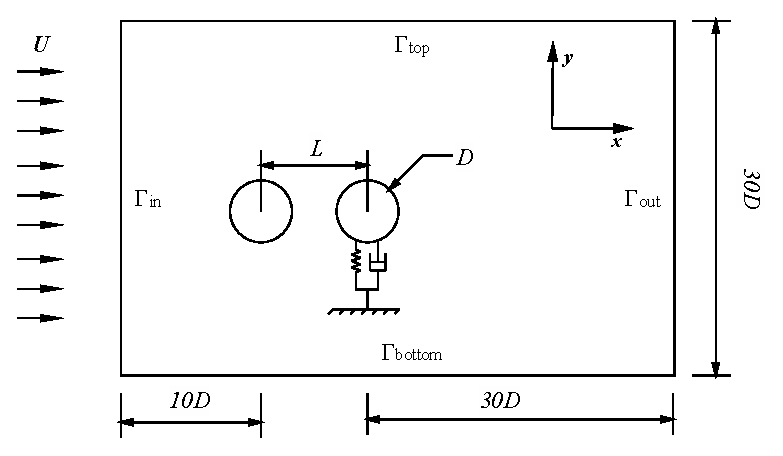
\includegraphics[scale=0.7]{wiv}}
     \caption{Schematic diagram of a representative bluff body of 
     elastically mounted cylinder in the wake of stationary cylinder. 
     Computational domain and boundary conditions are shown.}
\label{fig:schematic}
\end{figure}

\begin{figure}
\centering 
\begin{subfigure}{0.495\textwidth}
\centering
  \makebox[0pt]{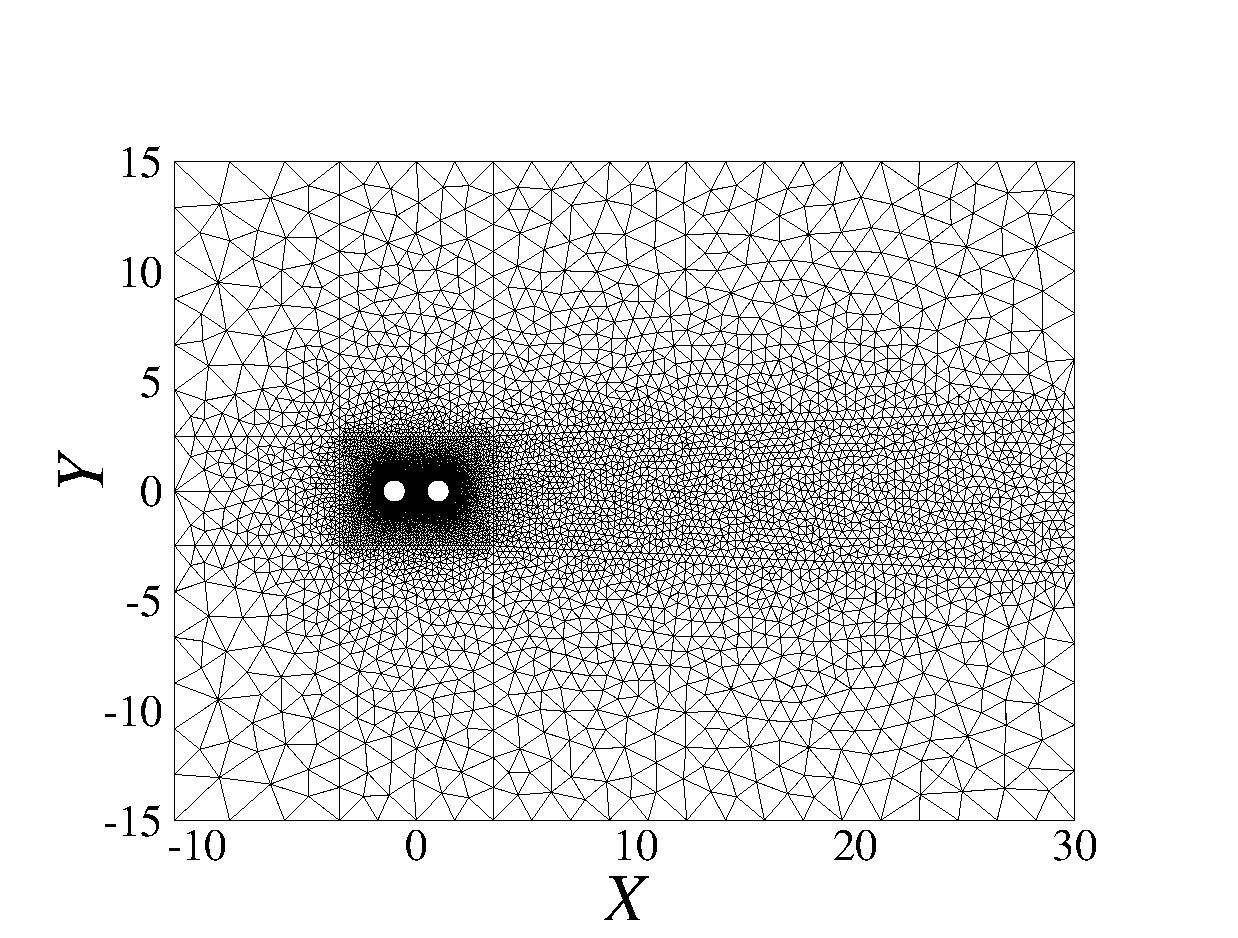
\includegraphics[scale=0.35]{mesh1}}
    \caption{}
    \label{•}
    \end{subfigure}  
\begin{subfigure}{0.495\textwidth}
\centering
  \makebox[0pt]{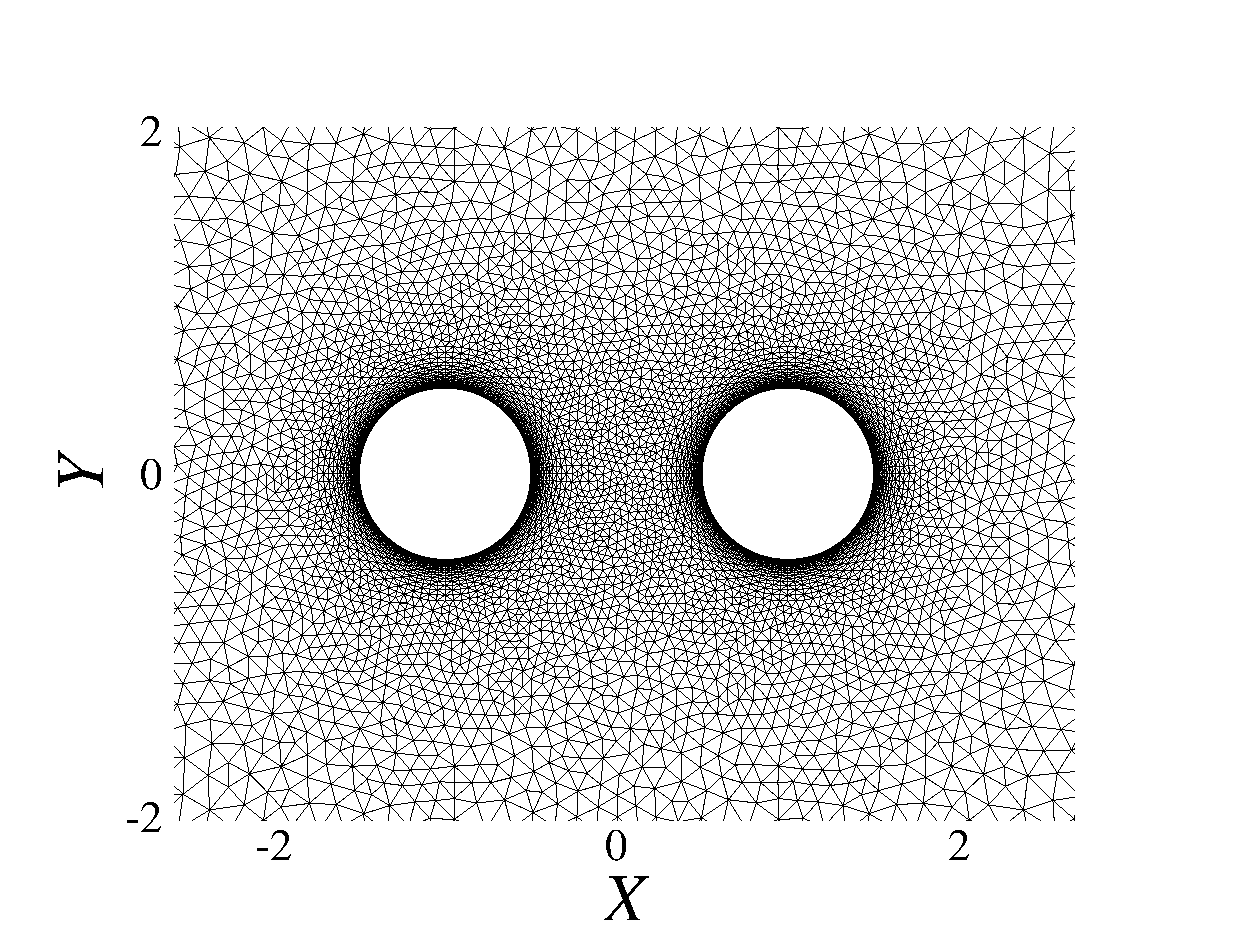
\includegraphics[scale=0.35]{mesh2}}
    \caption{}
    \label{•}
    \end{subfigure} 
  \caption{Finite element mesh with $\mathbb{P}_{2}/\mathbb{P}_{1}$ discretization: (a) full domain
discretization and (b) close-up view of in the vicinity of the
tandum cylinder. }
\label{fig:mesh}  
\end{figure}

\subsection{Stationary tandum cylinder linear stability analysis}\label{sec:lsa}

At $(Re,L)=(60,2D)$, the WIV ERA-based ROM is first constructed for circular cylinder 
tandum configuration. The based flow, as shown in the figure \ref{fig:baseflow}, is computed via fixed point iteration without the 
time dependent term in the NS equation. 
Following the ERA-based ROM construction procedure in \cite{yao_jfm_1}, 
1000 impulse outputs ($C_l$) are stacked by imposing $\delta (t) = 10^{-4}$
on the transverse displacement $Y$ of downstream cylinder with time step size $\Delta t = 0.05$.
Subsequently, $25^{th}$ ROM is determined by examining the decaying singular value of Hankel matrix \cite{Juang1985}. 
A good match between FOM and $25^{th}$ ROM is found in figure \ref{fig:signal}. The impulse response gradaully decays 
and indicates that real part of the least damped eigenvalue is negative and the uncoupled fluid system is stable. 
%
The least damped eigenvalue predictred by ERA-based ROM is compared with FOM in figure \ref{fig:fomeig}. The FOM results 
are derived by solving a generalized eigenvalue problem of Eq.~(\ref{eq:NS_pr}). 


\begin{figure}
	 \centering
	 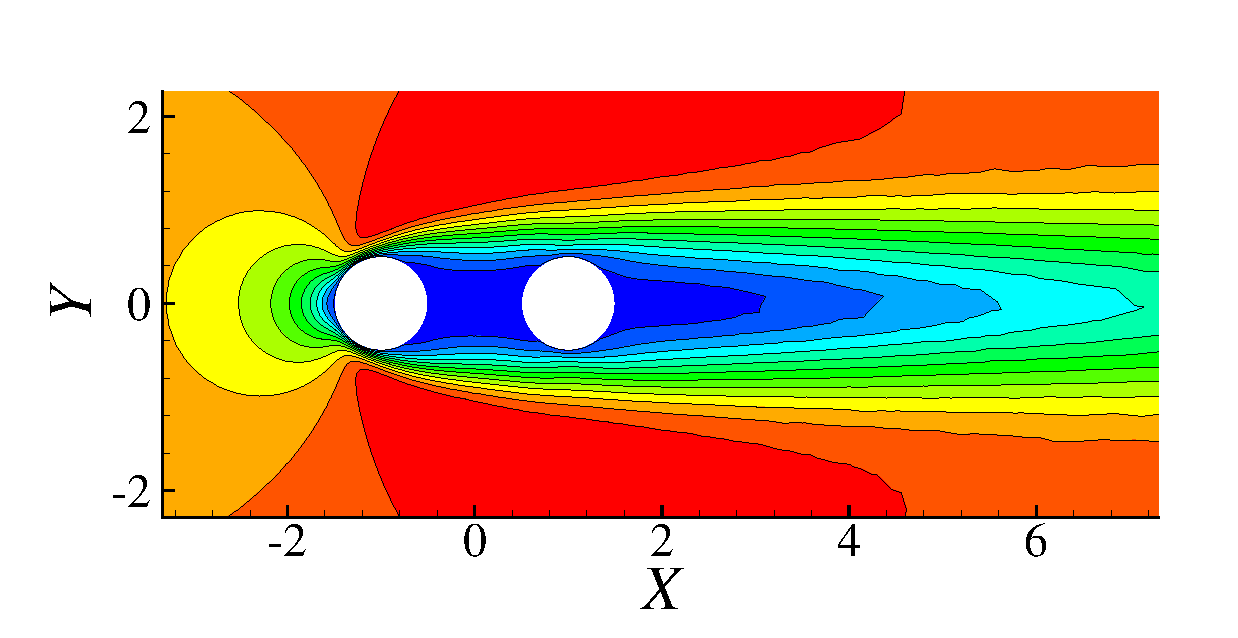
\includegraphics[scale=0.5]{baseflow_re60_ld2}
     \caption{Base flow of tandum circular cylinder at $(Re,L)=(60,2D)$; The 
     streamwise velocity contours are shown. The contour levels are from -0.1 to 1.2 
     in increments of 0.1.}
\label{fig:baseflow}
\end{figure}


\begin{figure}
\centering 
\begin{subfigure}{0.495\textwidth}
\centering
  \makebox[0pt]{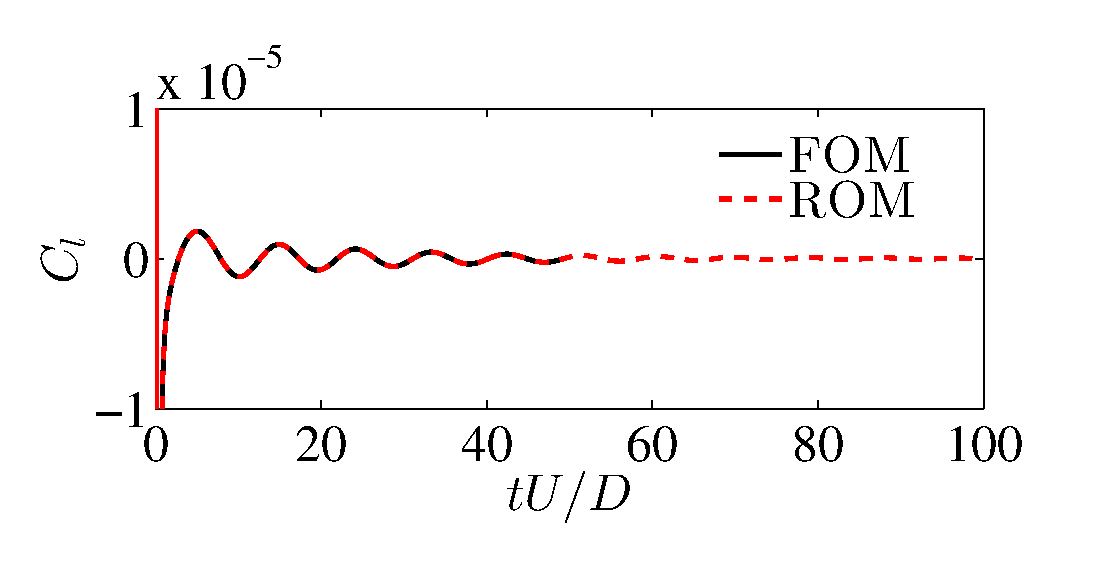
\includegraphics[scale=0.35]{signal}}
    \caption{}
    \label{•}
    \end{subfigure}  
\begin{subfigure}{0.495\textwidth}
\centering
  \makebox[0pt]{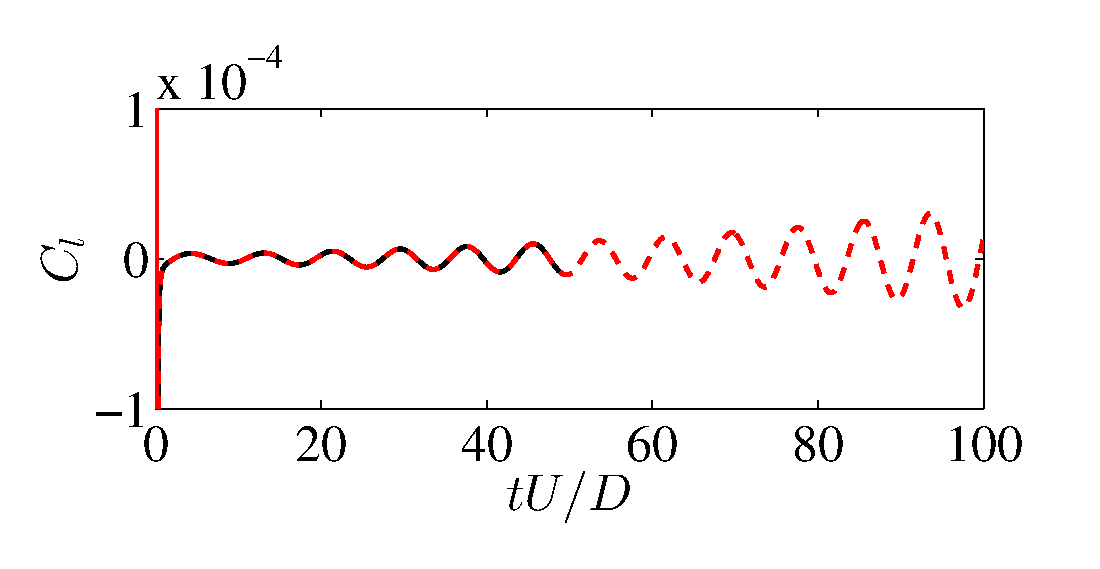
\includegraphics[scale=0.35]{signalre120}}
    \caption{}
    \label{•}
    \end{subfigure} 
  \caption{The lift coefficient history of the $25^{th}$ 
     ROM compared with FOM subject to the impulse response.
     (a) $Re=60$. (b) $Re=120$. }
\label{fig:signal}  
\end{figure}

%

\begin{figure}
	 \centering
	 \makebox[0pt]{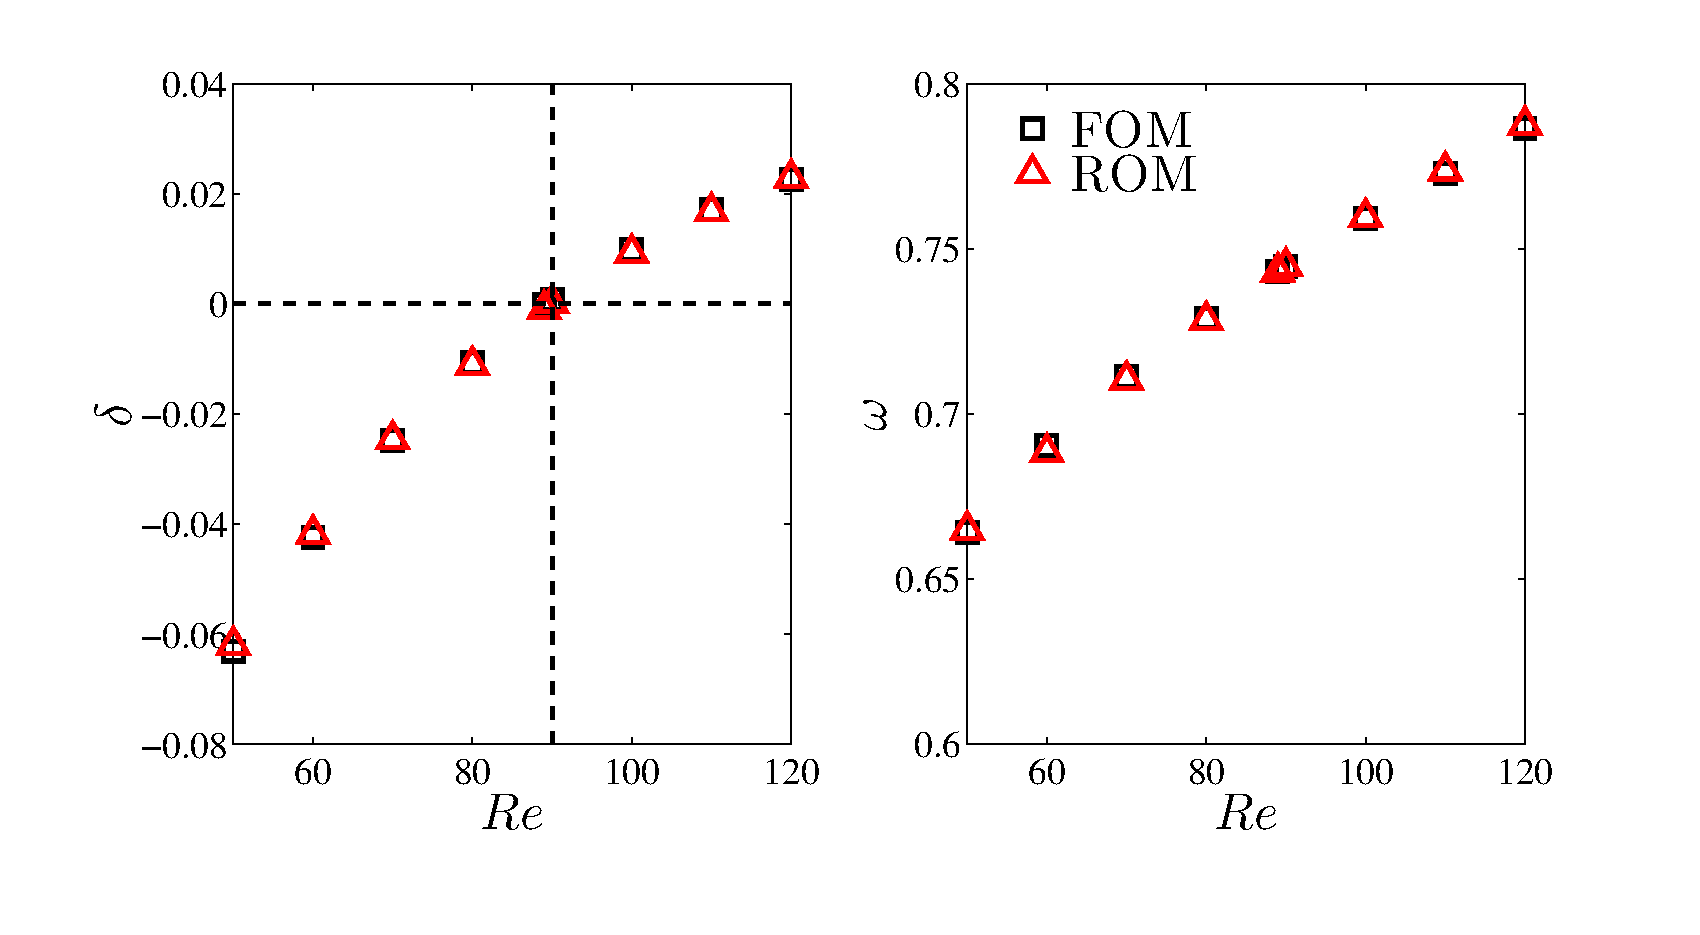
\includegraphics[scale=0.5]{fomeig}}
     \caption{The growth rate and frequency of the least damped eigenvalue for the 
                flow past a tandum circular cylinder with $L=2D$: 
                (a) growth rate $\sigma$ and
                (b) frequency $\omega$.  The cylinder wake becomes unstable when 
                the growth rate crosses $\sigma=0$ line at the critical 
                $Re_{cr} \approx 90$ and the vortex shedding emanates. }
\label{fig:fomeig}
\end{figure}



\section{Results and discussion}\label{sec:Results}
\subsection{WIV of circular cylinder}\label{sec:WIV_circular}

%%

Figure \ref{fig:ld2_eig} shows the root loci of the WIV ERA-based ROM as a function of reduced 
velocity $U_r$ with $2 \le U_r \le 40$. Following previous work in \cite{yao_jfm_1}, the terminology 
WMI and WMII are adopted to classify the eigenvalue branches. As can be seen, 
the WMII branch arises from the high frequency region or the top
of the complex plane, while the WMI branch originates from the uncoupled mode and travels down to the low frequency 
or bottom of the complex plane. 
As elucidated in the figure \ref{fig:ld2_eig}, 
the real part of WMII branch remains unstable when $U_r \ge 6.1$ and WMI branch is stable, 
which indicates the WIV persists at $m^*=2$. The finding is further 
confirmed by the FOM in figure \ref{fig:fom_2_ycl}, where the WIV onset $U_r=5.9$ and the WIV remains for $U_r \ge 5.9$. 
Figure \ref{fig:ld2_eig} shows that the WMI branch is only unstable when $7.44 \le U_r \le 11.0$ at $m^*=20$, which is evident 
from the figure \ref{fig:fom_2_ycl}. 
Furthermore, in figure \ref{fig:ld2_eig}(b) (bottom), the Im$(\lambda)$ plot shows the charateristic anticrossing between WMI and WMII for 
the low mass ratio $m^*=2$. This intrinsic property of strong coupling system is also found for single cylinder VIV system at 
low mass ration \cite{yao_jfm_1}. 
The two counter-rotating vortices (2S mode) are released at onset $U_r=5.9$ and $(Re,m^*,L)=(60,2,2D)$ 
as shown in figure \ref{fig:fom_2_onset_vor}. 
%% response 
The figure \ref{fig:m2_fom} and \ref{fig:m20_fom} depict the transverse displacement and lift traces with the 
corresponding spectrum, which confirms the high harmonid response of WIV. 

%%

Apart from the unstable eigenvalue branches, it is also interesting to see the WIV from the engergy transfer viewpoint.
The engery transfer over one period $T$ for WIV system is derived as equation \ref{eq:Energy_transfer} 
in Appendix A. The $E_c$ is defined by excluding the exponential growth/decay rate. The figure \ref{fig:energy} suggests 
that energy source to sustain the WIV is the unstable WMII at $(Re,L)=(60,2D)$. 
 
\begin{figure}
\centering 
\begin{subfigure}{0.495\textwidth}
\centering
  \makebox[0pt]{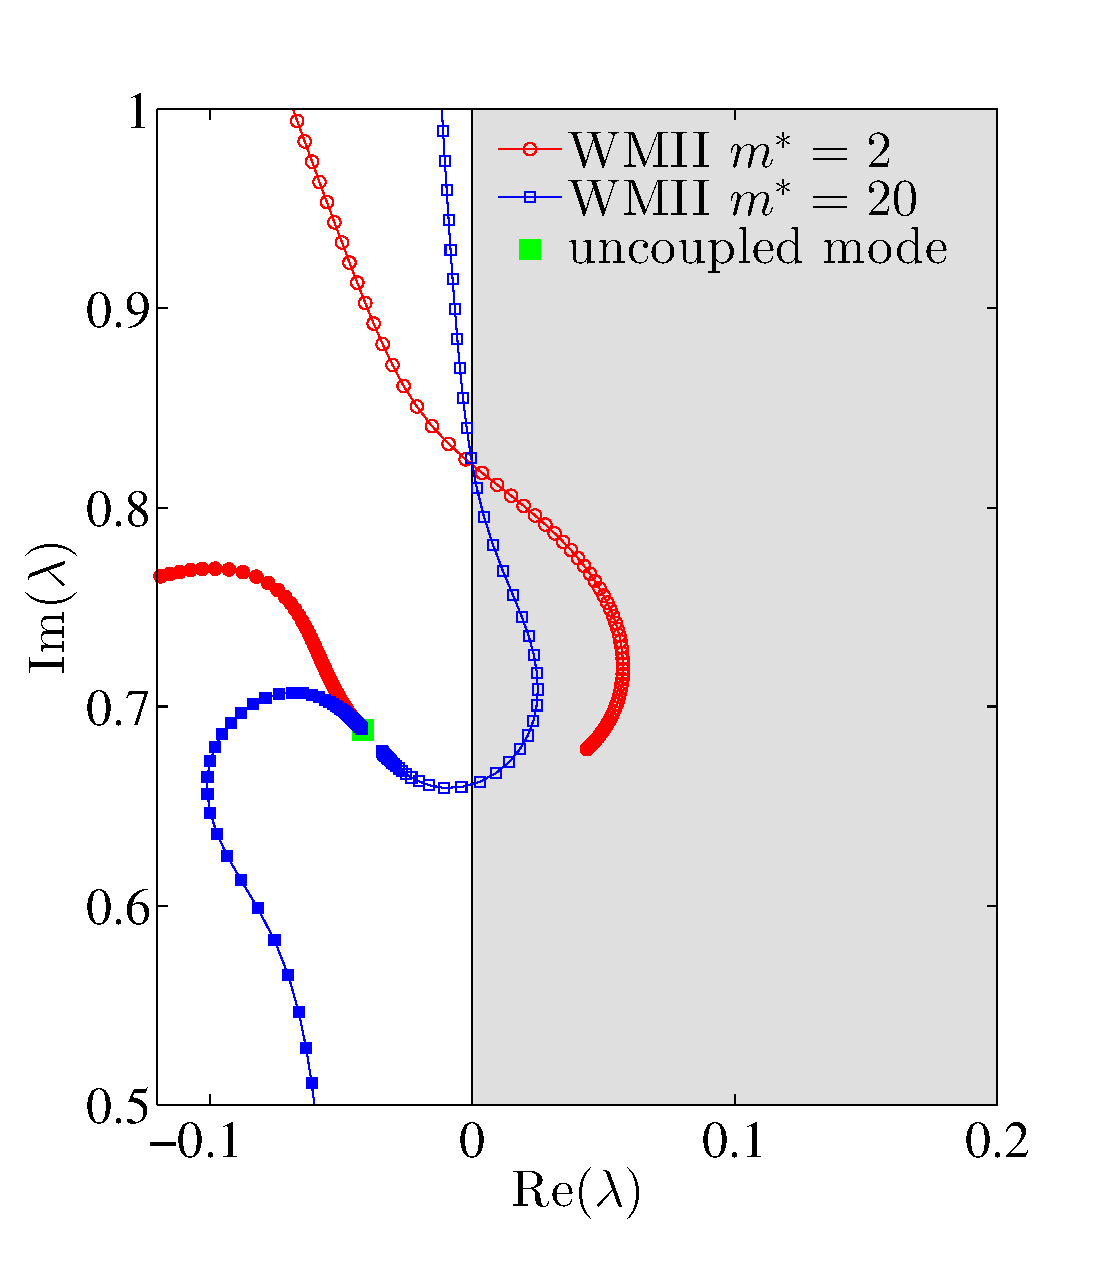
\includegraphics[scale=0.35]{eig1_re60_mstar}}
    \caption{}
    \label{•}
    \end{subfigure}  
\begin{subfigure}{0.495\textwidth}
\centering
  \makebox[0pt]{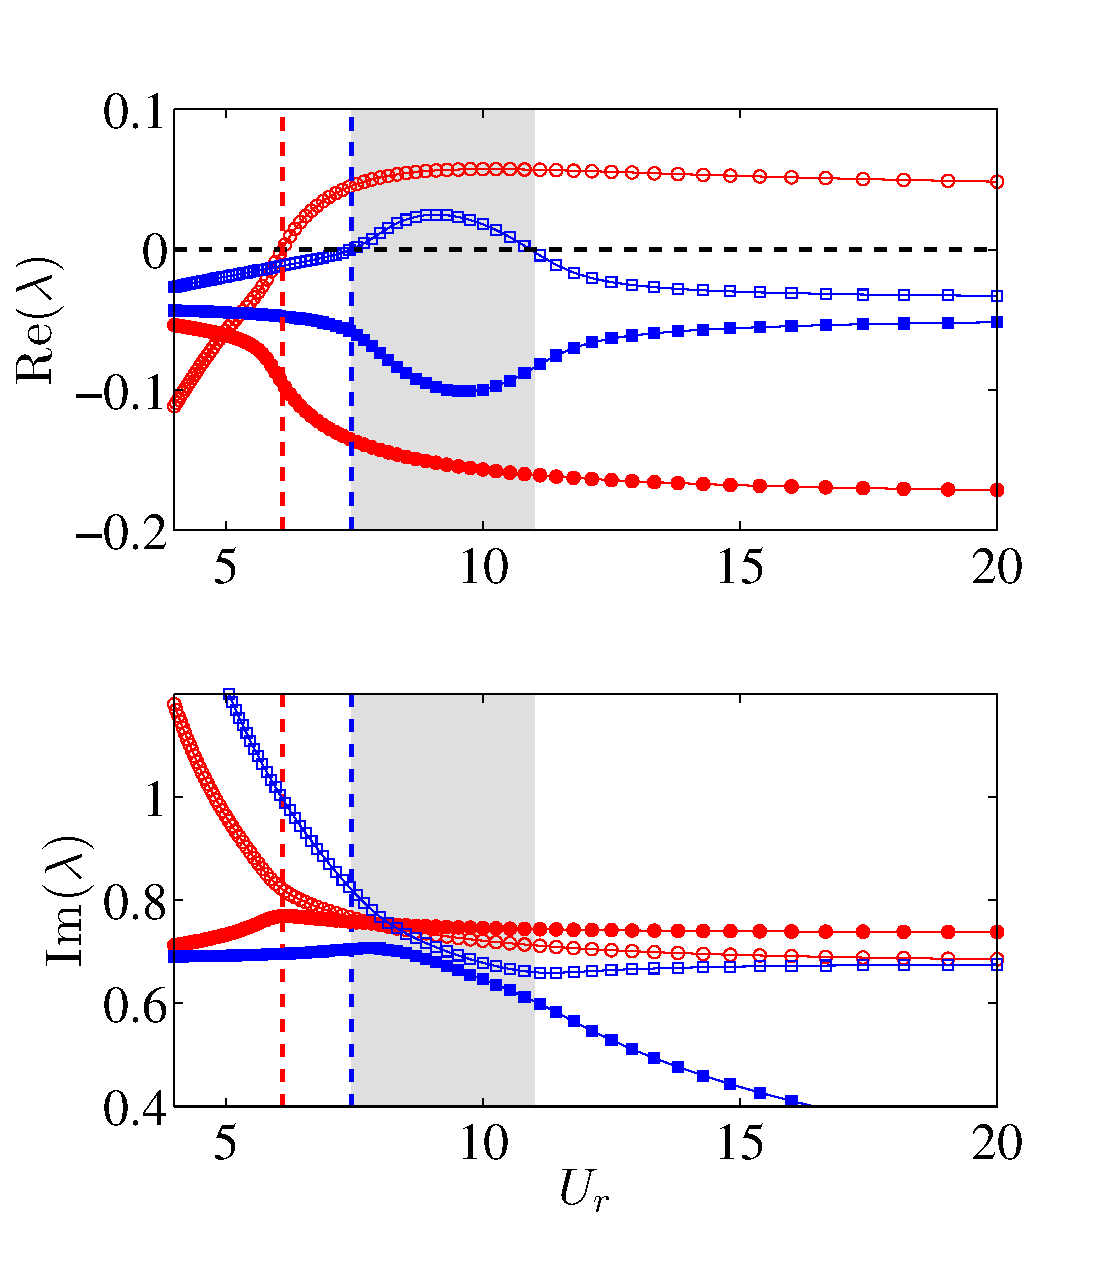
\includegraphics[scale=0.35]{eig2_re60_mstar2_20}}
    \caption{}
    \label{•}
    \end{subfigure} 
  \caption{Eigenspectrum of the ERA-based ROM at $(Re,L)=(60,2D)$: 
     (a) root loci as a function of the reduced velocity $U_r$, 
     where the unstable right-half (Re$(\lambda) > 0$) plane is shaded in grey color.
     The WMI is denoted by filled symbols with the same shape as those for the WMII. 
     The uncouled wake mode $\lambda=-0.042+0.69i$.
     (b) Real and imaginary parts of the root loci at $(Re,L)=(60,2D)$.
     The WIV region at $m^*=20$ is shaded in grey colour, which is defined by 
     $7.44 \le U_{r} \le 11.0$.
     {\protect\reddash} and {\protect\bluedash} represent WIV onset $U_r \approx 6.1$ 
      and $U_r \approx 7.44$ for $m^*=(2,20)$, respectively.}
\label{fig:ld2_eig}  
\end{figure}


%% mstar = 2

\begin{figure}
	 \centering
	 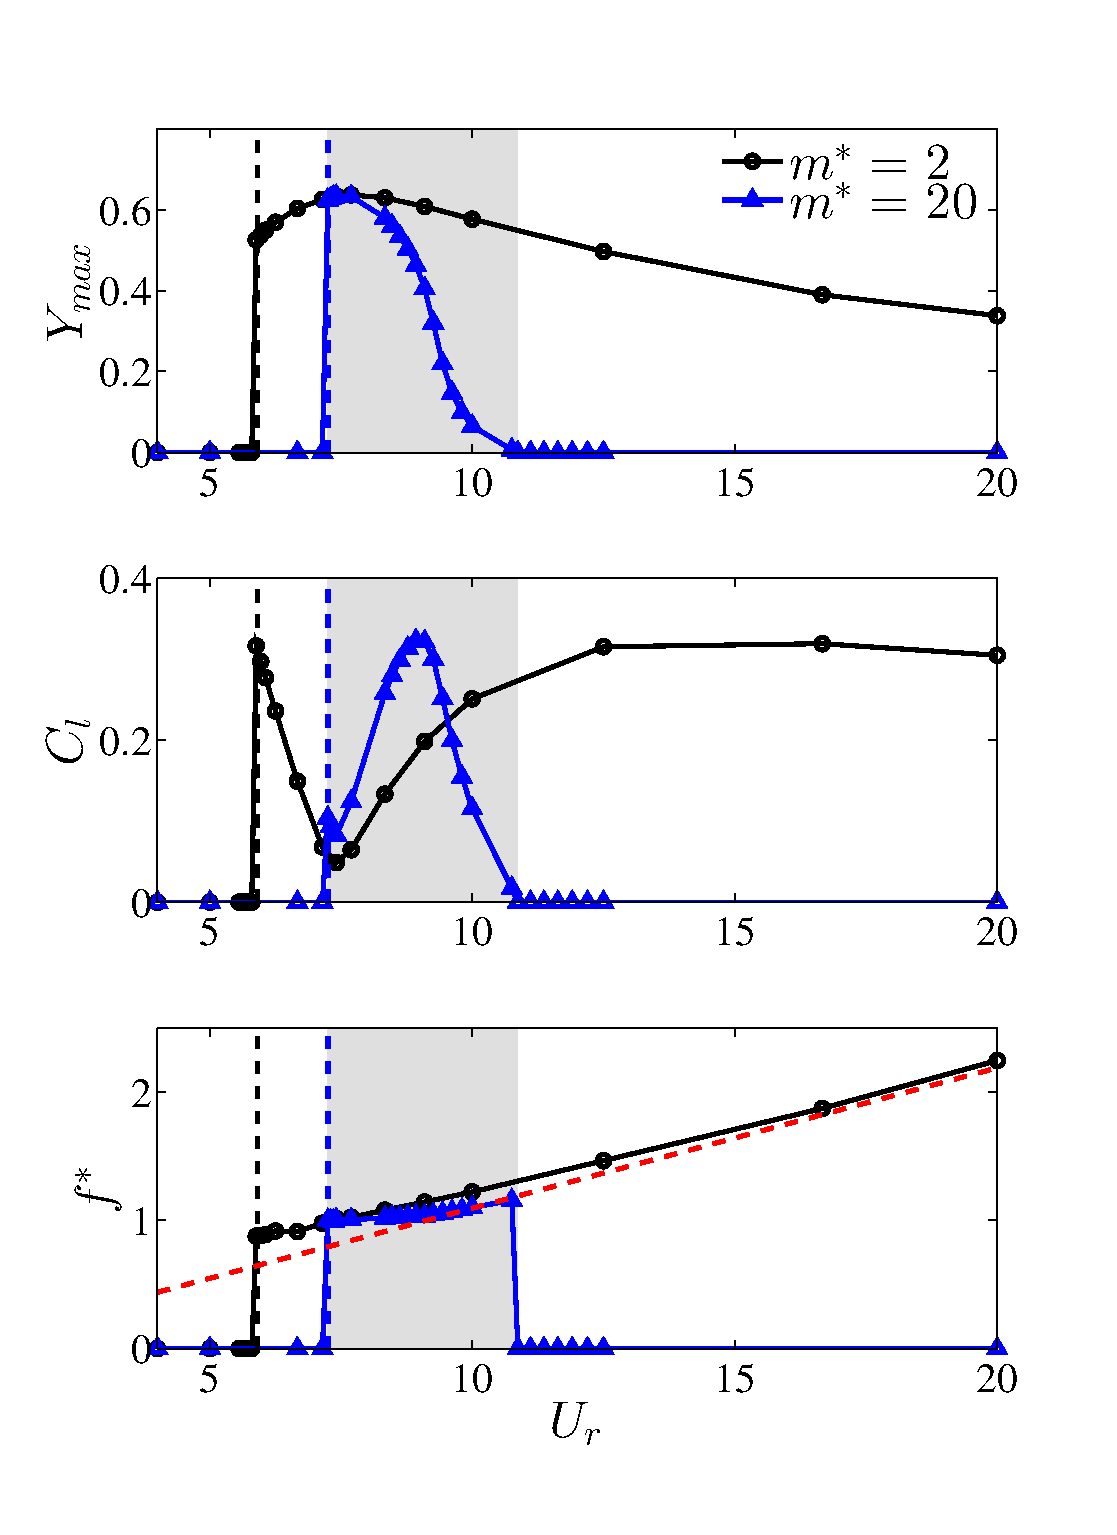
\includegraphics[scale=0.45]{fom_circle_m2_20}
     \caption{Normalized maximum amplitude $Y_{max}$ and 
        rms value of lift coefficient $C_l$
         as a function of reduced velocity $U_r$ at $(L,Re)=(2D,60)$. 
        The WIV region $7.25 \le U_{r} \le 10.87$ at $m^*=20$ is shaded in grey colour.
        {\protect\blackdash} and {\protect\bluedash} represent WIV onset $U_r=5.9$ 
        and $U_r=7.25$, respectively. {\protect\reddash} is the uncoupled mode frequency predicted by ROM.}
\label{fig:fom_2_ycl}
\end{figure}



\begin{figure}
	 \centering
	 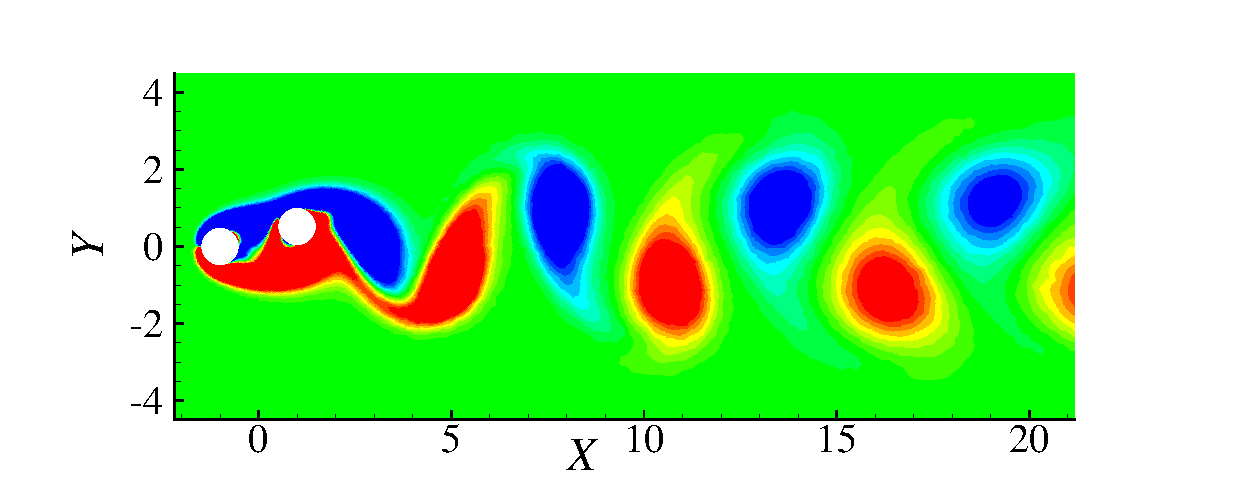
\includegraphics[scale=0.45]{circle_re60_m2_onset_vor}
     \caption{Instantaneous vorticity contours of WIV onset ($U_r=7.25$)
      at $(Re,m^*,L)=(60,2,2D)$.
      The contour levels are from −0.5 to 0.5 in increments of 0.067 and the flow is from left to
      right. }
\label{fig:fom_2_onset_vor}
\end{figure}
%%
\begin{figure}
\centering
\begin{subfigure}{0.495\textwidth}
\centering
  \makebox[0pt]{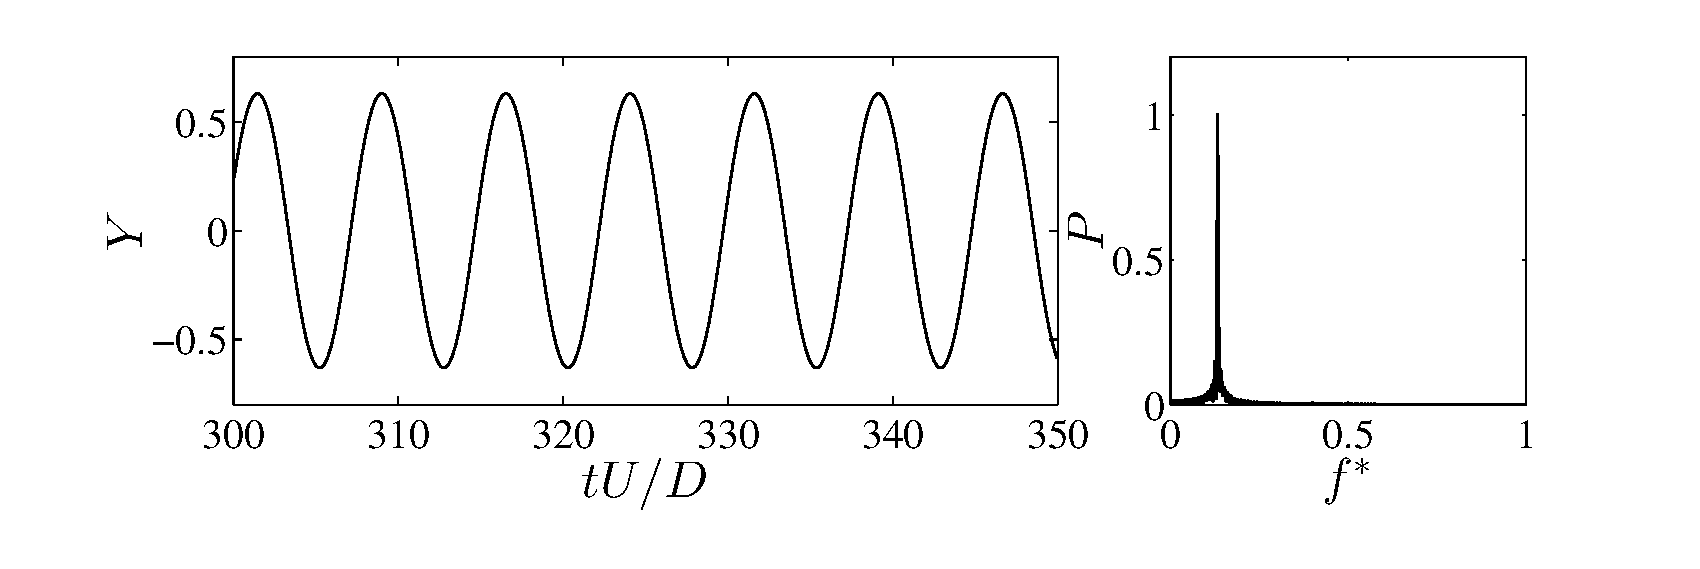
\includegraphics[scale=0.45]{m2_fom_yy_peak}}
    \caption{}
    \label{fig:yy}
    \end{subfigure} \\
\begin{subfigure}{0.495\textwidth}
\centering
   \makebox[0pt]{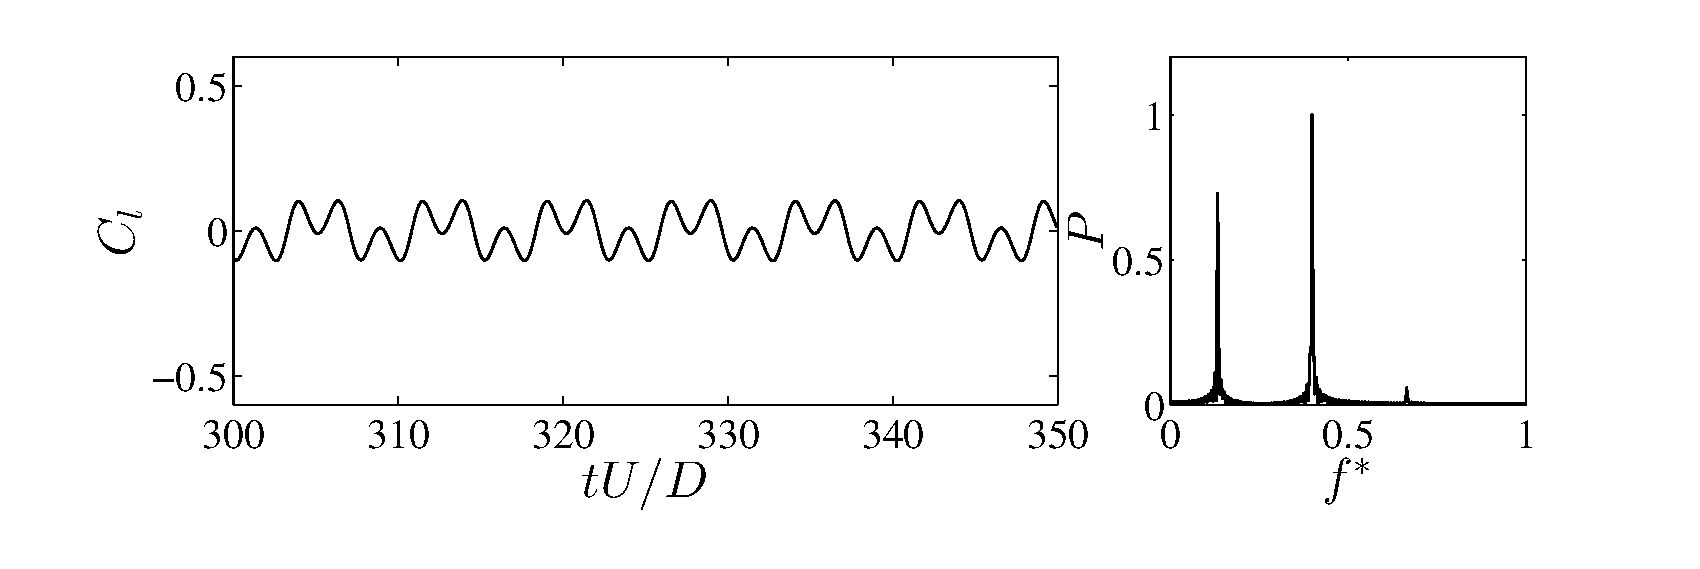
\includegraphics[scale=0.45]{m2_fom_cl_peak}}
    \caption{}
    \label{fig:cl}
    \end{subfigure} 
  \caption{FOM results of circular WIV at $(Re,m^*,L)=(60,2,2D)$:
        temporal variation of 
        (a) transverse amplitude, and (b) lift coefficient; 
        normalized power spectrum $P$ versus $f^*$ of: 
        (a) transverse amplitude, (b) lift coefficient at reduced velocity $U_r \approx 7.69$ or $F_s=0.13$, where  $f^*=f/F_s$ 
        is the frequency of lift and transverse displacement normalized 
        by reduced natural frequency $F_s$. 
        A third-harmonic frequency is evident in $C_l$.}
\label{fig:m2_fom}  
\end{figure}
%%
\begin{figure}
\centering
\begin{subfigure}{0.495\textwidth}
\centering
  \makebox[0pt]{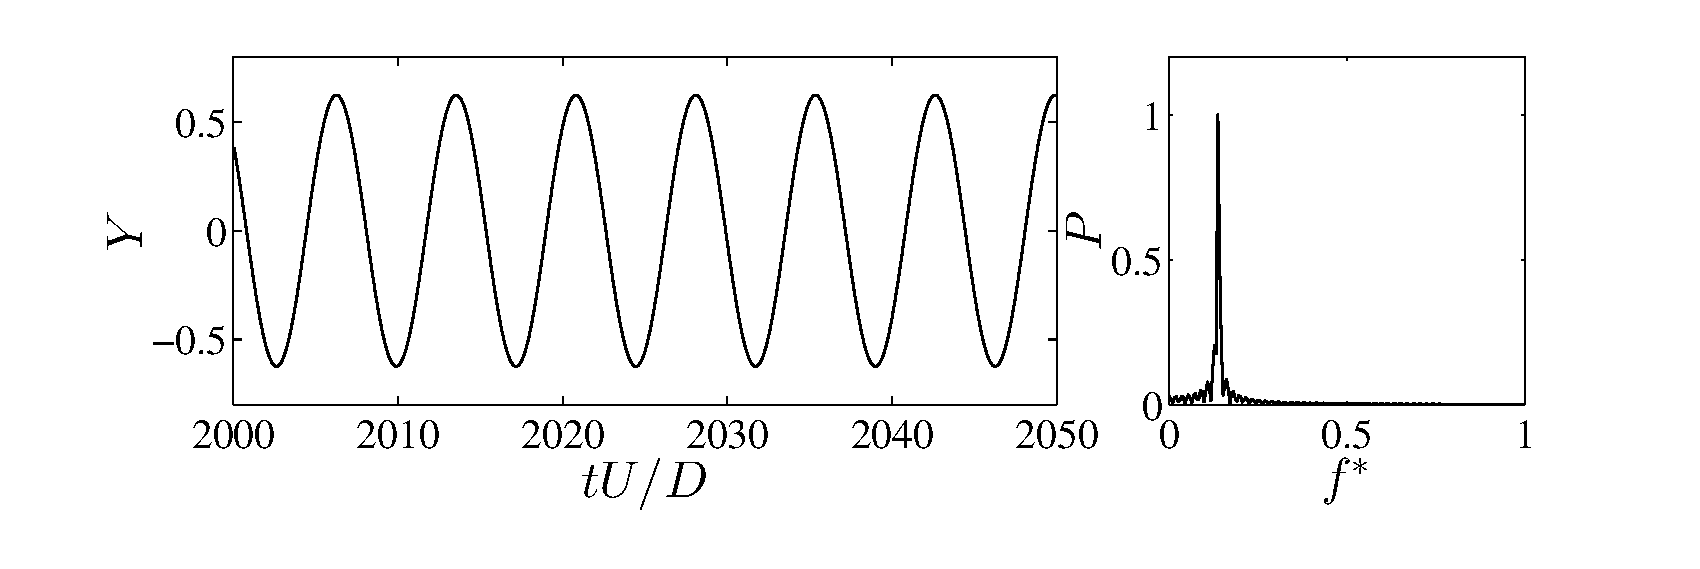
\includegraphics[scale=0.45]{m20_fom_yy_onset}}
    \caption{}
    \label{fig:yy}
    \end{subfigure} \\
\begin{subfigure}{0.495\textwidth}
\centering
   \makebox[0pt]{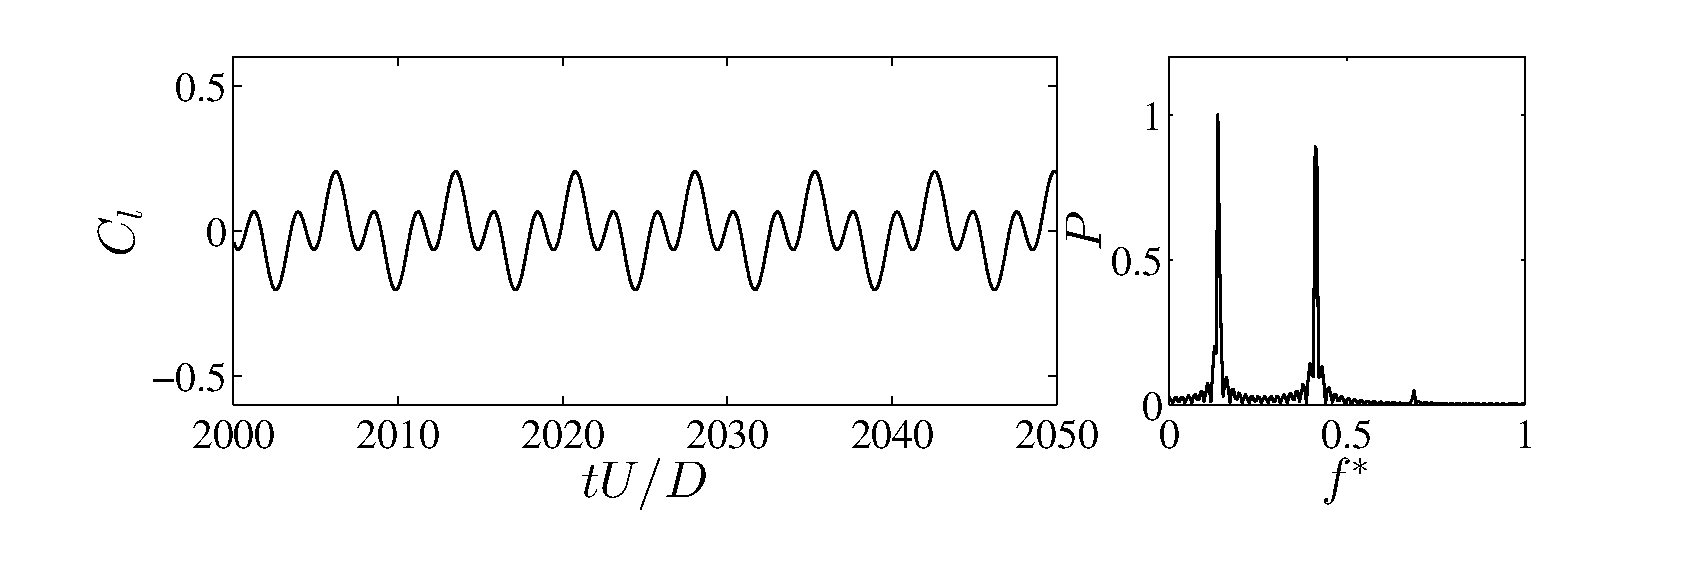
\includegraphics[scale=0.45]{m20_fom_cl_onset}}
    \caption{}
    \label{fig:cl}
    \end{subfigure} 
  \caption{FOM results of circular WIV at $(Re,m^*,L)=(60,20,2D)$:
        temporal variation of 
        (a) transverse amplitude, and (b) lift coefficient; 
        normalized power spectrum $P$ versus $f^*$ of: 
        (a) transverse amplitude, (b) lift coefficient at onset reduced velocity $U_r \approx 7.25$ or $F_s=0.138$, where  $f^*=f/F_s$ 
        is the frequency of lift and transverse displacement normalized 
        by reduced natural frequency $F_s$. 
        A third-harmonic frequency is evident in $C_l$.}
\label{fig:m20_fom}  
\end{figure}


% energy 
\begin{figure}
\centering 
\begin{subfigure}{0.495\textwidth}
\centering
  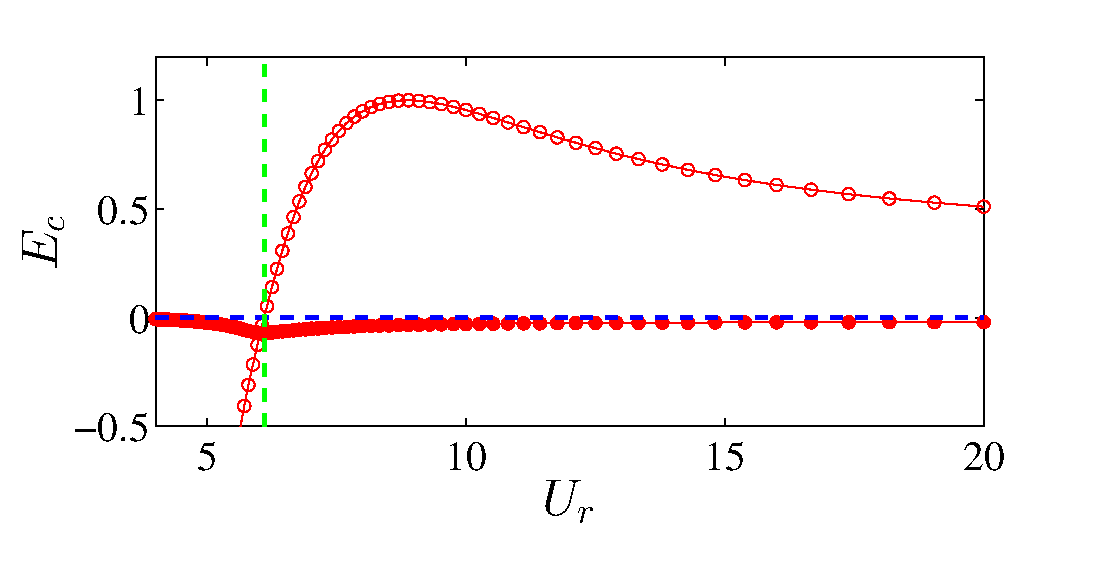
\includegraphics[scale=0.45]{Ec_re60_mstar2}
    \caption{}
    \label{fig:Ec_m2}
    \end{subfigure}  \\
\begin{subfigure}{0.495\textwidth}
\centering
  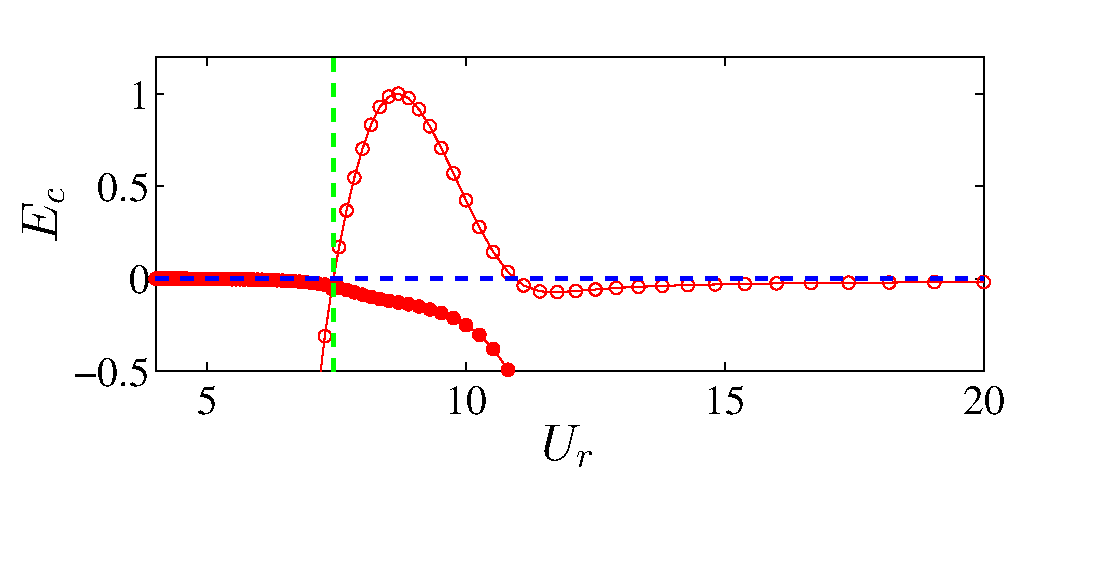
\includegraphics[scale=0.45]{Ec_re60_mstar20}
    \caption{}
    \label{fig:Ec_m20}
    \end{subfigure} 
  \caption{$E_c$ as a function of reduced velocity $U_r$ at $(L,Re)=(2D,60)$.
  (a) $m^*=2$, and (b) $m^*=20$. {\protect\greendash} represents the onset reduced velocity $U_r$.}
\label{fig:energy}  
\end{figure}

%%

As shown \ref{fig:ld2_eig_re100}, the uncoupled mode moves to the right half-complex-plane at $Re=100$. 
Compared with root loci at $Re=60$, figure \ref{fig:ld2_eig_re100} shows that the eigenvalue branches 
moves to high frequency regime or upper part of complex plane. The onset $U_r$ of WIV predicted by ERA-based ROM 
is at $U_r \approx 5.4$.  
Figure \ref{fig:fom_20_onset_vor} shows the instantaneous vortex structure at onset reduced velocity $U_r \approx 5.3$
which shows C(2S) pattern. 



\begin{figure}
\centering 
\begin{subfigure}{0.495\textwidth}
\centering
  \makebox[0pt]{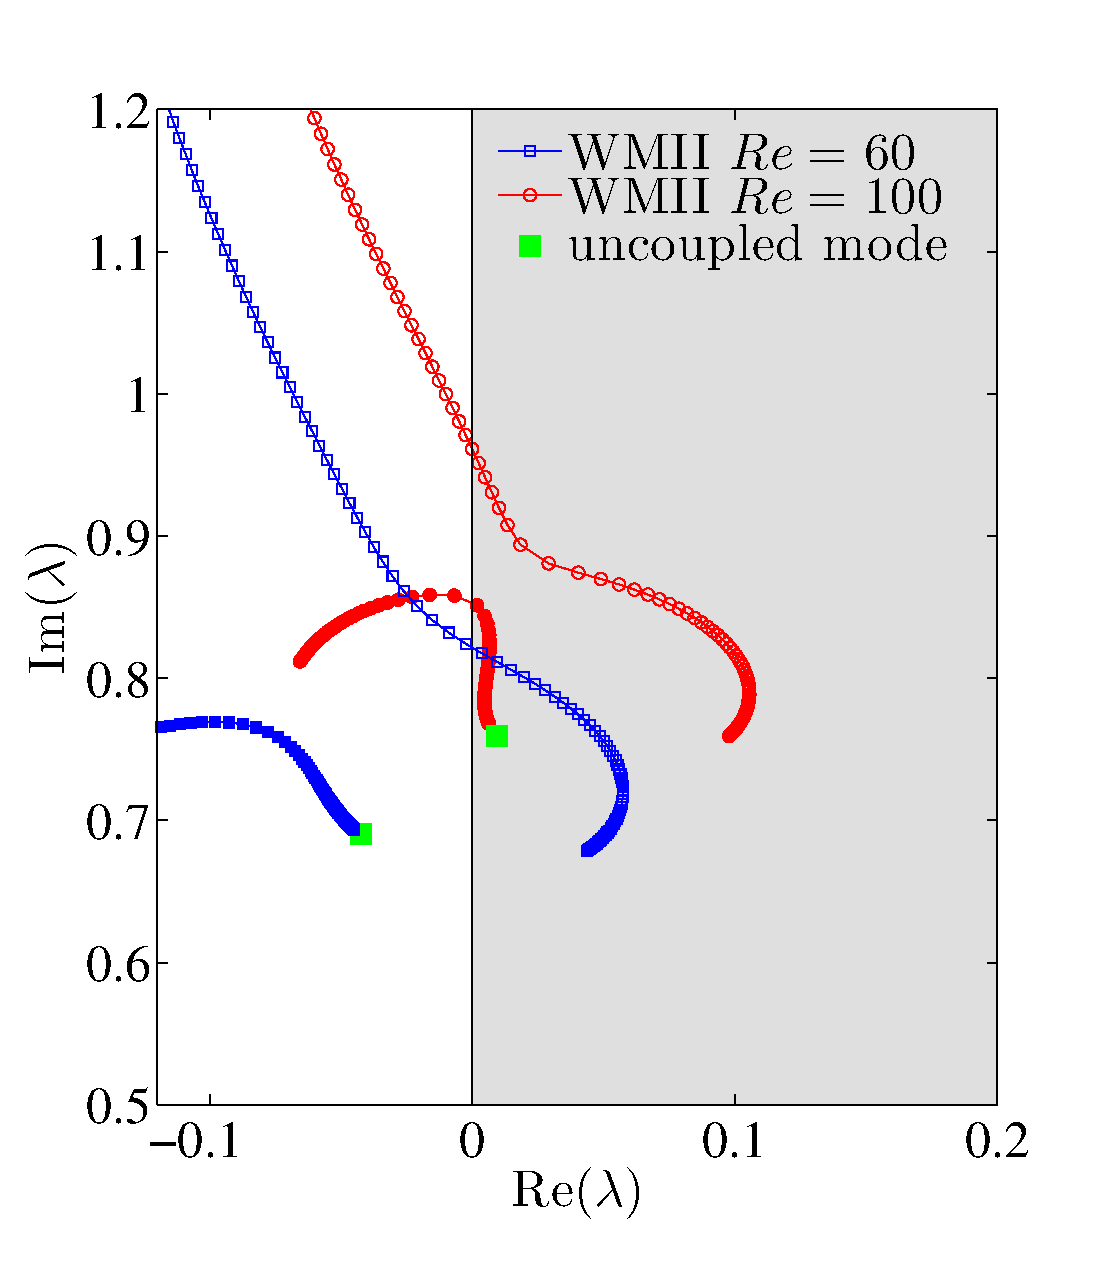
\includegraphics[scale=0.35]{eig1_re100_mstar}}
    \caption{}
    \label{•}
    \end{subfigure}  
\begin{subfigure}{0.495\textwidth}
\centering
  \makebox[0pt]{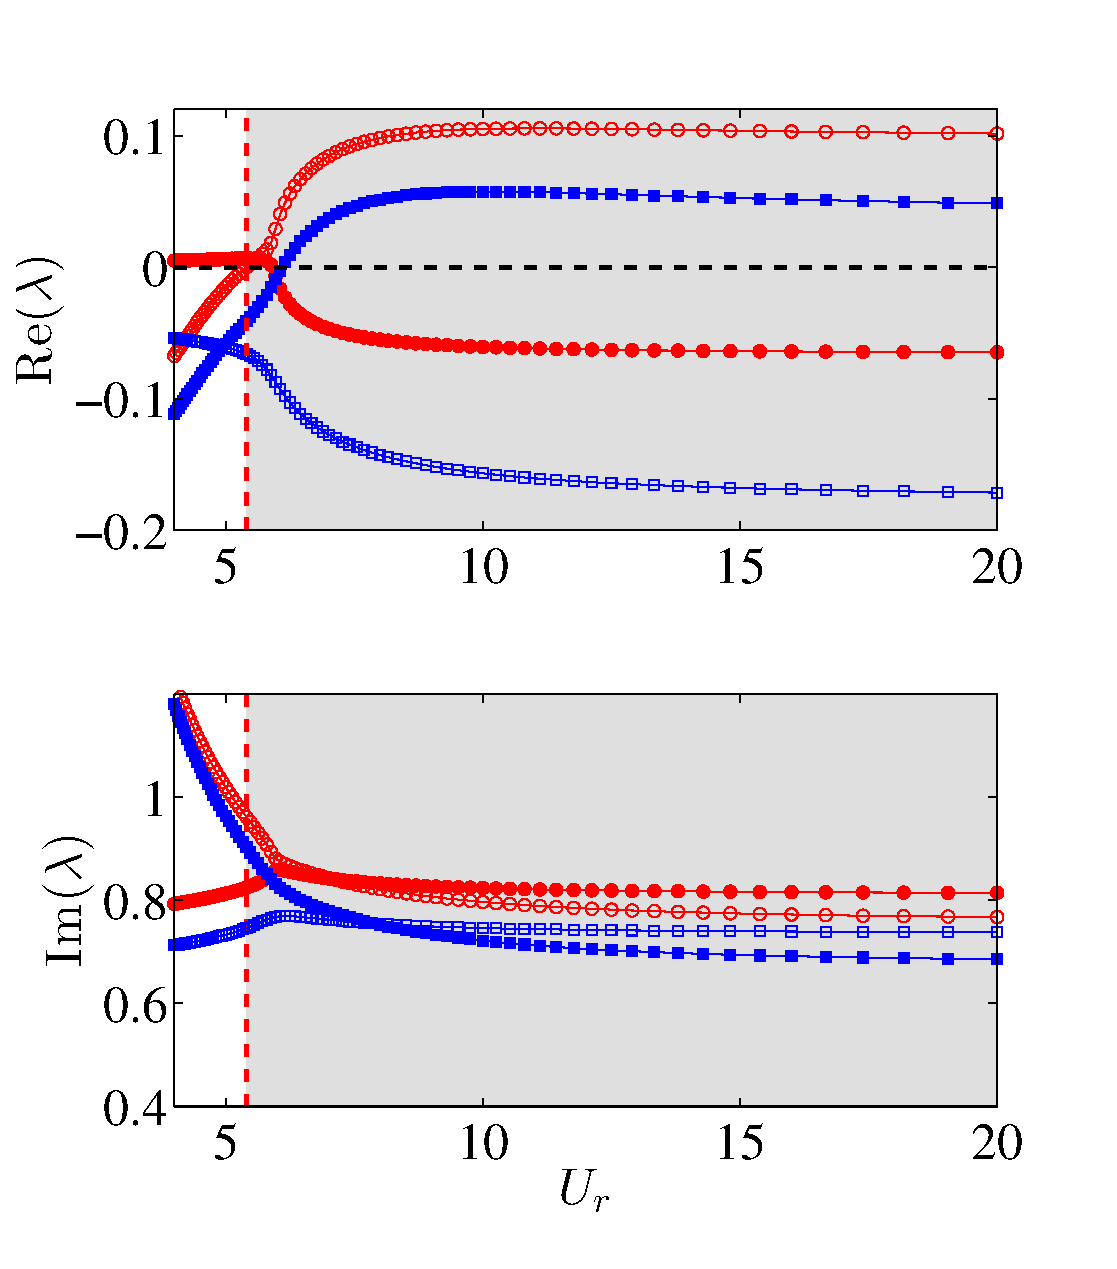
\includegraphics[scale=0.35]{eig2_re100_mstar}}
    \caption{}
    \label{•}
    \end{subfigure} 
  \caption{Eigenspectrum of the ERA-based ROM at $(m^*,L)=(2,2D)$: 
     (a) root loci as a function of the reduced velocity $U_r$, 
     where the unstable right-half (Re$(\lambda) > 0$) plane is shaded in grey color.
     The WMI is denoted by filled symbols with the same shape as those for the WMII. 
     The uncouled wake mode $\lambda=0.01+0.759i$.
     (b) Real and imaginary parts of the root loci at $(Re,L)=(100,2D)$.
     The WIV region at $(Re,m^*)=(100,2)$ is shaded in grey colour, which is defined by 
     $ U_{r} \ge 5.4$.}
\label{fig:ld2_eig_re100}  
\end{figure}

%%
\begin{figure}
	 \centering
	 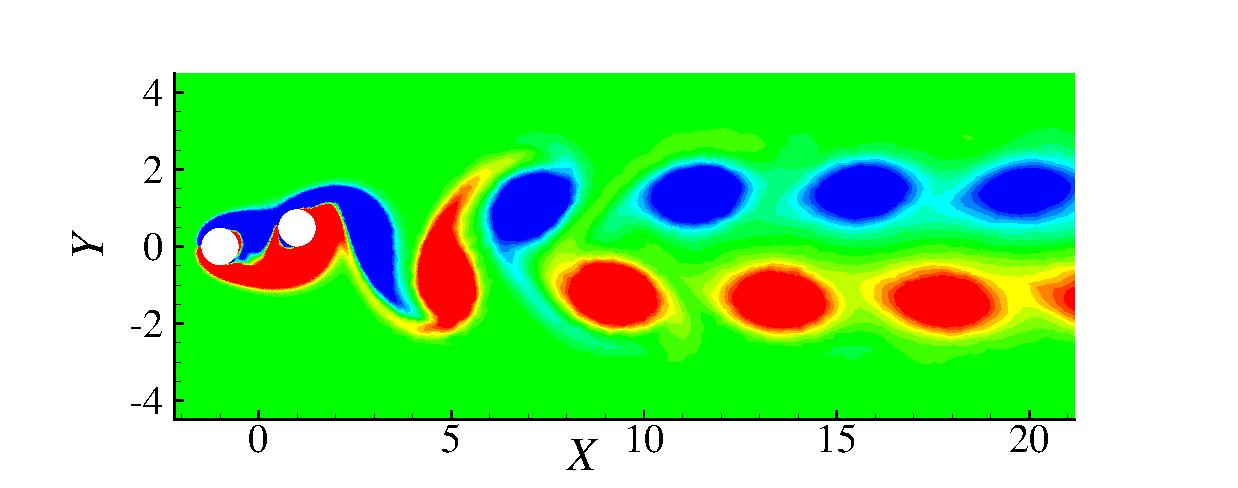
\includegraphics[scale=0.45]{circle_re100_m2_onset_vor}
     \caption{Instantaneous vorticity contours of WIV onset ($U_r=5.3$)
      at $(Re,m^*,L)=(100,2,2D)$.
      The contour levels are from −0.5 to 0.5 in increments of 0.067 and the flow is from left to
      right. }
\label{fig:fom_20_onset_vor}
\end{figure}

\subsection{WIV of square cylinder}\label{sec:WIV_square}

In this section, we further explore the WIV of square cylinder. In our previous work \cite{yao_jfm_1}, 
we demonstrates that the sharp corner has stabilizing effects for fluid strucutre coupling. Thereofre, 
It is interesting to investigate the WIV mechanism of square cylinder by means of ERA-based ROM.
The flow region with high sensitivity and strong response or wavemaker region is determined by computing the pointwise 
product of the forward and adjoint global modes \cite{Luchini2007}. 
Figure \ref{fig:wavemaker} shows that the wavemaker region of the circular tandum cylinder has higher value and 
moves closer to the cylinders than its circular counterpart, which suggests that the circular tandum cylinder 
has stronger fluid and structure interation level. 


\begin{figure}
\centering 
\begin{subfigure}{0.495\textwidth}
\centering
  \makebox[0pt]{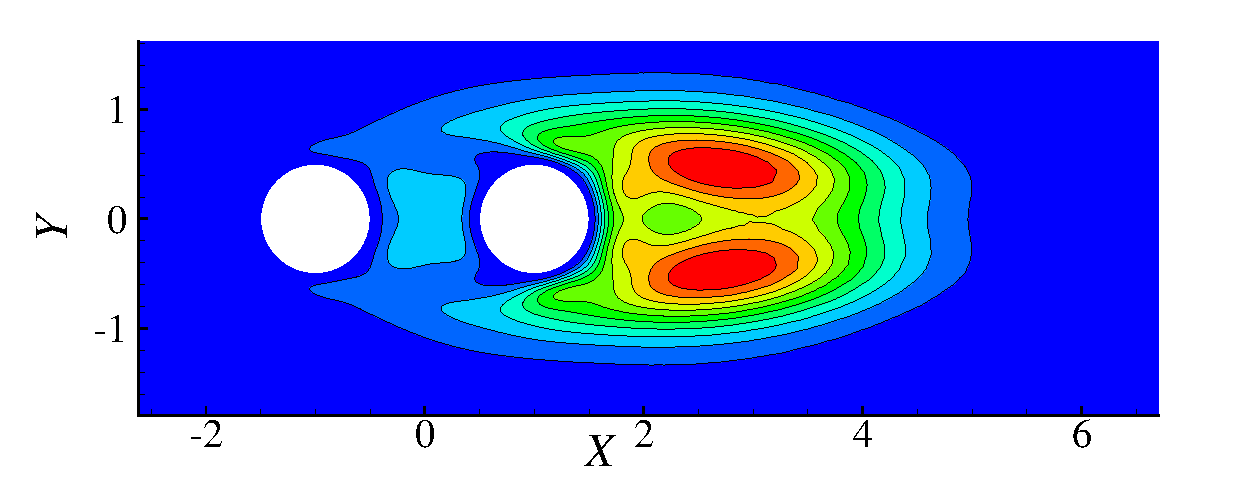
\includegraphics[scale=0.35]{wavemaker_circle_re60}}
    \caption{}
    \label{fig:wavemaker_circle}
    \end{subfigure} 
\begin{subfigure}{0.495\textwidth}
\centering
  \makebox[0pt]{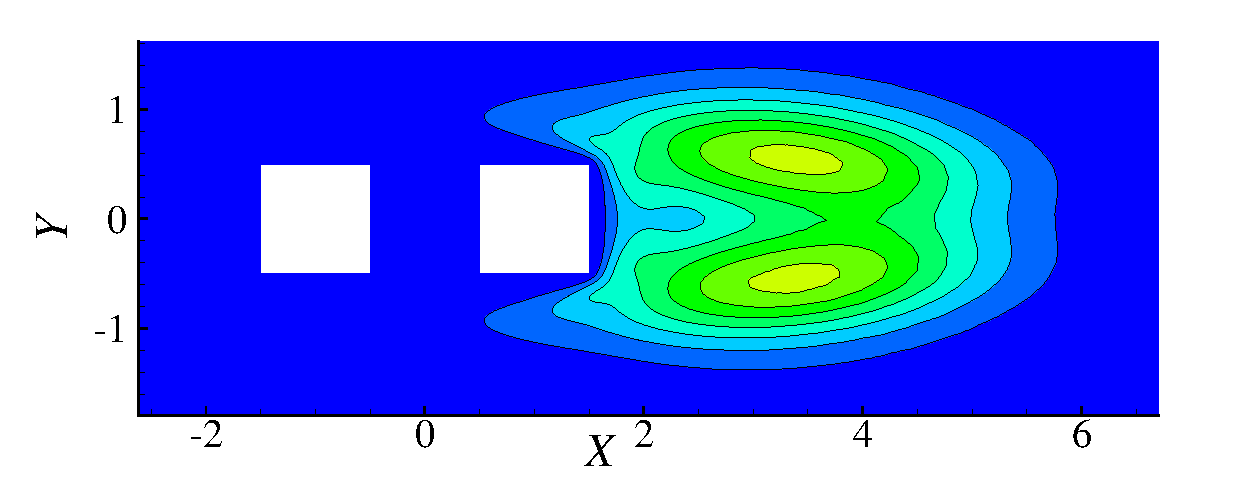
\includegraphics[scale=0.35]{wavemaker_square_re60}}
    \caption{}
    \label{fig:wavemaker_square}
    \end{subfigure} 
  \caption{Wavemaker region of (a) circular and (b) square cylinder at $(Re,L)=(60,2D)$.
  The contour levels are from 0.04 to 0.35 in increments of 0.035 and the flow is from left to right. }
\label{fig:wavemaker}  
\end{figure}




%%%%%%%%%% square wiv
%% 
\begin{figure}
\centering 
\begin{subfigure}{0.495\textwidth}
\centering
  \makebox[0pt]{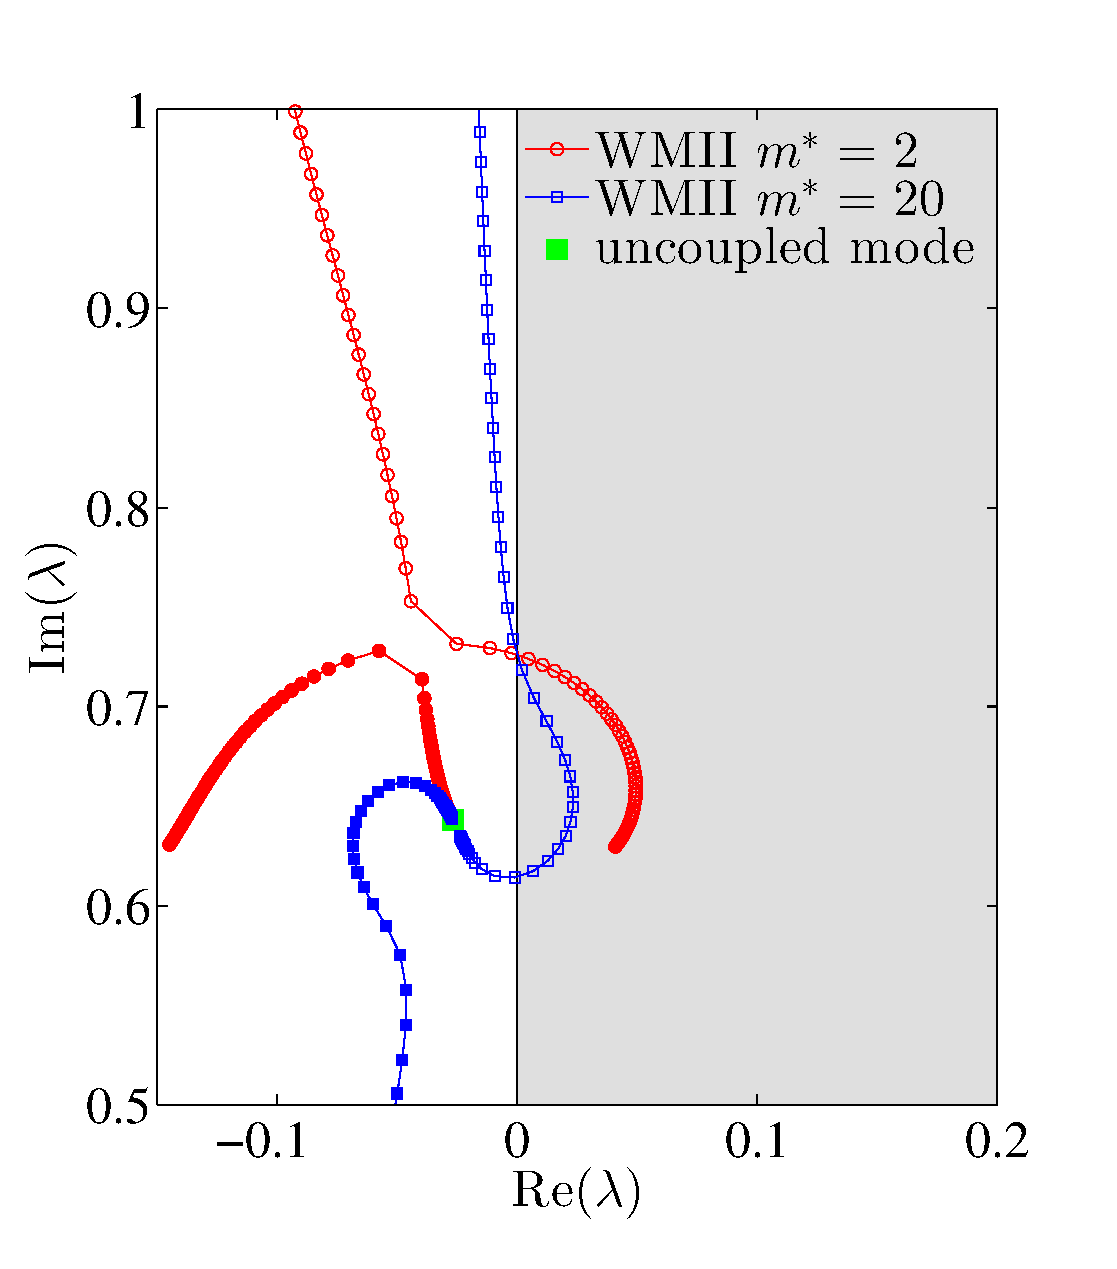
\includegraphics[scale=0.35]{eig1_re60_mstar_square}}
    \caption{}
    \label{•}
    \end{subfigure}  
\begin{subfigure}{0.495\textwidth}
\centering
  \makebox[0pt]{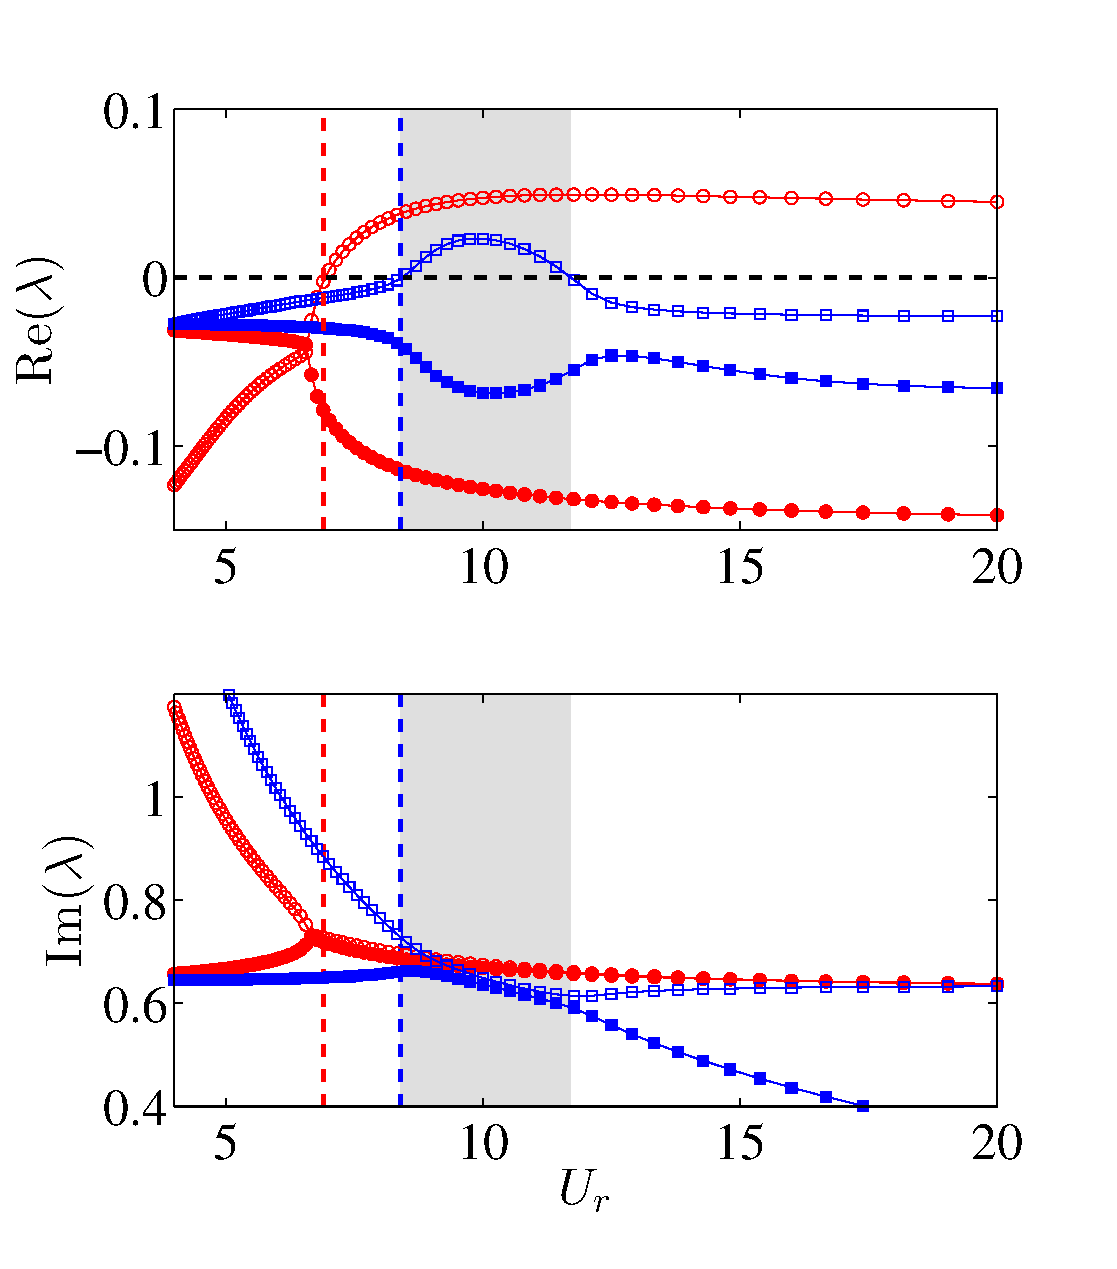
\includegraphics[scale=0.35]{eig2_re60_mstar_square}}
    \caption{}
    \label{•}
    \end{subfigure} 
  \caption{Eigenspectrum of the ERA-based ROM at $(Re,L)=(60,2D)$: 
     (a) root loci as a function of the reduced velocity $U_r$, 
     where the unstable right-half (Re$(\lambda) > 0$) plane is shaded in grey color.
     The WMI is denoted by filled symbols with the same shape as those for the WMII. 
     The uncouled wake mode $\lambda=-0.027+0.643i$.
     (b) Real and imaginary parts of the root loci at $(Re,L)=(60,2D)$.
     The WIV region at $m^*=20$ is shaded in grey colour, which is defined by 
     $8.4 \le U_{r} \le 11.7$.
     {\protect\reddash} and {\protect\bluedash} represent WIV onset $U_r=6.75$ 
      and $U_r=8.4$ for $m^*=(2,20)$, respectively.}
\label{fig:ld2_eig_square}  
\end{figure}



%% mstar = 2

\begin{figure}
	 \centering
	 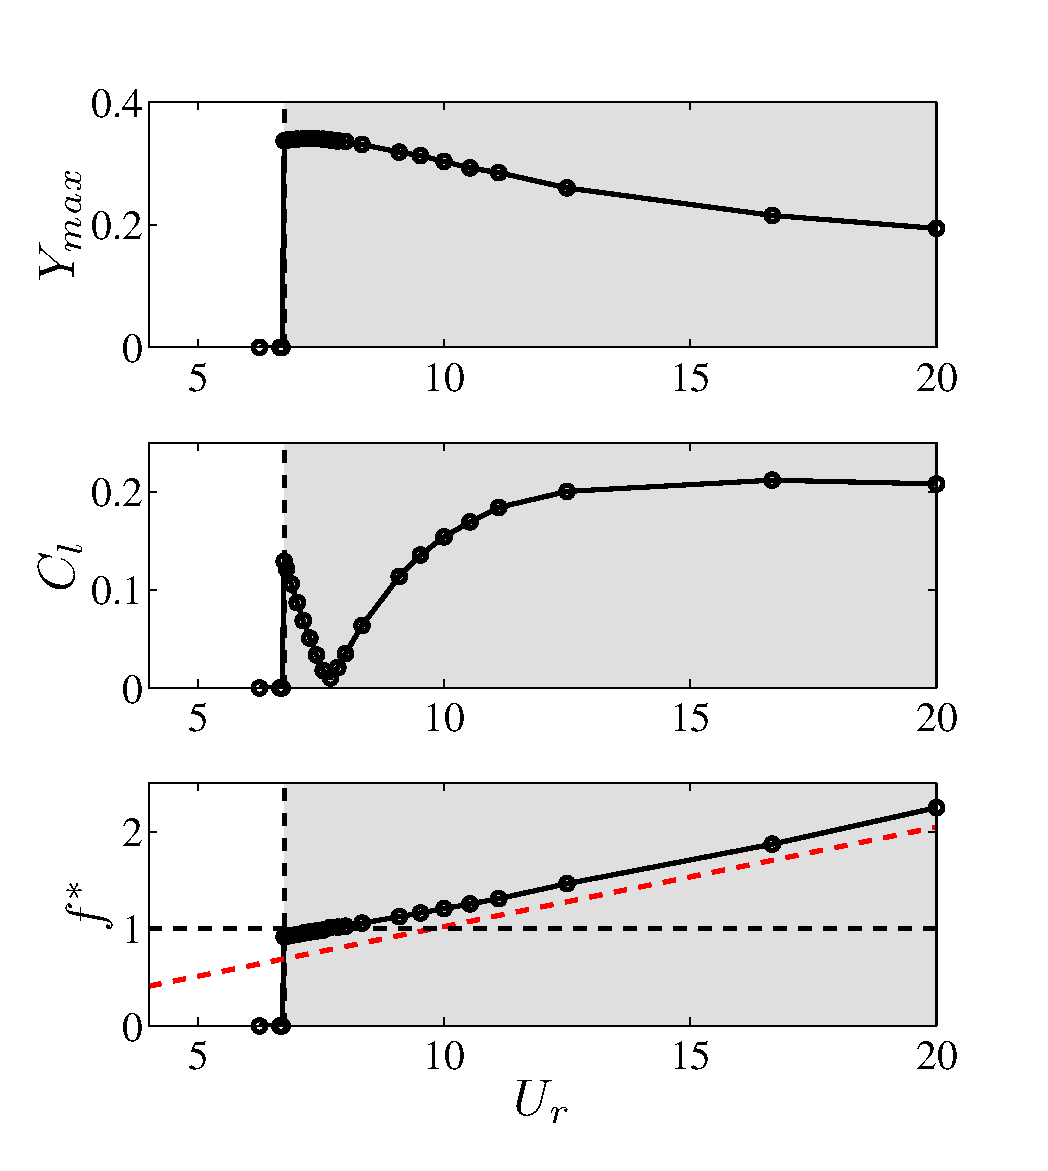
\includegraphics[scale=0.45]{fom_square_m2}
     \caption{Normalized maximum amplitude $Y_{max}$ and 
        rms value of lift coefficient $C_l$
         as a function of reduced velocity $U_r$ at $(L,Re,m^*)=(2D,60,2)$. 
        The WIV region is shaded in grey colour.
        {\protect\blackdash} represents WIV onset $U_r=6.76$. {\protect\reddash} is the uncoupled WM frequency predicted by ROM. }
\label{fig:fom_2_ycl}
\end{figure}
%%
\begin{figure}
	 \centering
	 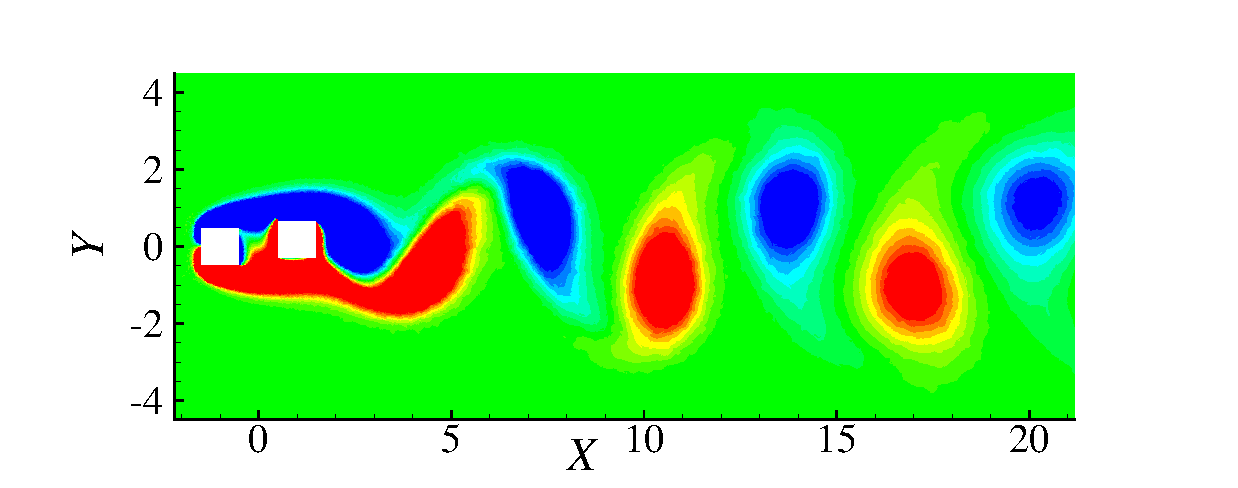
\includegraphics[scale=0.45]{square_re60_m2_onset_vor}
     \caption{Instantaneous vorticity contours of WIV onset ($U_r=6.76$)
      at $(L,Re,m^*)=(2D,60,2)$.
      The contour levels are from −0.5 to 0.5 in increments of 0.067 and the flow is from left to
      right. }
\label{fig:fom_20_onset_vor}
\end{figure}


\section{Concluding remarks}




\section*{Appendix A: Energy Transfer for WIV}\label{app:A} 

Following our previous work on VIV \cite{yao_jfm_1}, 
the displacement and lift coefficient can be obtained  for the WIV linear system as, 
 
\begin{equation}
\left. \begin{array}{ll}
\displaystyle Y=\hat{Y} e^{\lambda_r t}\cos(\lambda_i t)  \\[8pt]
\displaystyle C_l=\hat{C_l} e^{\lambda_r t}\cos(\lambda_i t + \phi)
\end{array}\right\},
\label{eq:linear_y_cl}
\end{equation}
where $\lambda=\lambda_r+i\lambda_i$ is eigenvalue with real $\lambda_r$ 
and imaginary $\lambda_i$ components, $\hat{Y}$ and $\hat{C_l}$ 
denote the magnitudes of eigenmodes. The phase angle difference is derived 
by pluging the Eq. (\ref{eq:linear_y_cl}) into Eq. (\ref{eq:structure1}), and refer
to \cite{yao_jfm_1} for details. 

\begin{equation}
\sin{\phi} = \frac{2\lambda_r\lambda_i}{\sqrt{(\lambda_r^2  \\
+ (2\pi F_s)^2 + \lambda_i^2)^2 - (4\pi\lambda_i F_s)^2 }}.
\label{eq:phase_angle}
\end{equation}

The engery transfer per cycle is defined as,

\begin{equation}
\begin{array}{ll}
\displaystyle E(t) = \int_{t}^{t+\frac{2 \pi}{\lambda_i}} \dot{Y} \hat{C_l} dt \\
\displaystyle  = \frac{1}{2}(\lambda_i \sin(\phi) + \lambda_r \cos(\phi) + \lambda_r \cos(2 \lambda_i t + \phi))
\int_{t}^{t+\frac{2 \pi}{\lambda_i}} e^{2 \lambda_r t} dt
\end{array}
\label{eq:Energy_transfer}
\end{equation}

$E_c$ is defined by excluding the exponential growth/decay rate $\lambda_r$ in Eq. (\ref{eq:Energy_transfer}),
\begin{equation}
E_c = \pi \hat{Y} \hat{C_l} \sin(\phi)
\end{equation}


%\begin{acknowledgements}
%If you'd like to thank anyone, place your comments here
%and remove the percent signs.
%\end{acknowledgements}

% BibTeX users please use one of
%\bibliographystyle{spbasic}      % basic style, author-year citations
\bibliographystyle{spmpsci}      % mathematics and physical sciences
%\bibliographystyle{spphys}       % APS-like style for physics
\bibliography{refs}   % name your BibTeX data base

% Non-BibTeX users please use
%\begin{thebibliography}{}
%%
%% and use \bibitem to create references. Consult the Instructions
%% for authors for reference list style.
%%
%\bibitem{RefJ}
%% Format for Journal Reference
%Author, Article title, Journal, Volume, page numbers (year)
%% Format for books
%\bibitem{RefB}
%Author, Book title, page numbers. Publisher, place (year)
%% etc
%\end{thebibliography}


\end{document}
% end of file template.tex

%\grid
